\chapter{Invitation: From Old Quantum Theory to Quantum States}
\begin{note}
    This chapter is introductory in character. It surveys the historical and experimental route from the crises of classical physics to the modern notion of the quantum state, and it presupposes nothing beyond classical mechanics, electromagnetism, and elementary thermodynamics. Subsections marked with a star contain optional derivations; they may be skipped on a first reading without loss of continuity.
\end{note}
The development of Quantum Mechanics as it is can be roughly divided into two phases: that of the \textbf{Old Quantum Theory} and that of the \textbf{Modern Quantum Mechanics}, of which, the latter in particular will be discussed in this note. Nevertheless, the author considers it helpful for the reader to review, at least briefly, the historical development of both. This is not merely for practical orientation, although many readers may be content with a purely formal treatment of quantum mechanics. Rather, the historical path also helps reveal the conceptual difficulties that gave rise to the modern theory.

The author further maintains that such a study contributes not only to a better understanding of the physical nature of quantum mechanics, but also, for the believing reader, to a renewed wonder at the providence of the Creator, who brought all things into being \textit{ex nihilo} and whose creative command is poetically recalled in the words \textit{Fiat lux}. For the sake of brevity, however, many details of the historical ``plot'' will be omitted. The main line of development will be retained insofar as it prepares the way for the modern formulation.

At the end of the nineteenth century, the basic architecture of physics appeared remarkably secure. Newtonian mechanics supplied the language of trajectories and forces; Maxwell's equations unified electricity, magnetism, and light; thermodynamics and statistical mechanics connected heat with molecular motion. The great confidence of the period did not come from naivete. It came from genuine success. Planetary motion, mechanical engineering, optics, electrical technology, and the kinetic theory of gases all suggested that nature was, at least in principle, intelligible by continuous fields and deterministic motion.

The anomalies that led to quantum mechanics were therefore especially disturbing. They were not merely small numerical disagreements. Black-body radiation, atomic spectra, and the photoelectric effect touched the foundations of energy exchange, radiation, and matter itself. The history of early quantum theory is the history of attempts to preserve as much of classical physics as possible while introducing just enough discontinuity to match experiment. Its greatness lies in this restraint; its limitation lies in the same place.

The narrative of this chapter is organized not by the calendar alone but by the crises that forced each new concept into existence. The first crisis concerned \emph{radiation and the exchange of energy}: the cavity spectrum, the photoelectric effect, and the specific heats of solids compelled the introduction of the energy quantum. The second crisis concerned \emph{the structure of the atom}: the discovery of the electron, Rutherford's nucleus, and the regularities of spectroscopy demanded a mechanics of stationary states, and received a provisional answer in the Bohr--Sommerfeld theory. The third crisis concerned \emph{waves, particles, and statistics}: Compton scattering, de Broglie's matter waves, Bose's counting, and the discovery of spin destroyed any hope that the quantum could be accommodated inside a classical ontology of particles and fields. Out of these three crises came the synthesis of 1925--1927: matrix mechanics, wave mechanics, the probability interpretation, and finally the representation-independent formalism of Dirac, Jordan, and von Neumann. The chapter closes by returning to the simplest experiments of all --- several of them older than the theory itself --- in which the new grammar of states and amplitudes can be read directly, preparing the systematic development of the following chapters.

\section{The First Crisis: Radiation and the Exchange of Energy}
Of the three crises, the crisis of radiation was chronologically the first and conceptually the deepest, because it arose inside the two most successful theories of the century. Cavity radiation is an electromagnetic problem; its equilibrium is a thermodynamic problem; its spectrum is a statistical problem. That a contradiction should appear precisely at the triple point of Maxwell's electromagnetism, thermodynamics, and Boltzmann's statistics was the first indication that the difficulty was not one of detail but of principle.

\subsection{Black-Body Radiation: the Classical Laws}
Thermal radiation is electromagnetic radiation emitted from the surface of an object due to the object's internal energy, which, traditionally, is treated by studying the radiation by the moving particles. If an object is heated sufficiently, it starts to emit light at the red end of the visible spectrum, as it becomes red hot. Heating it further causes the color to change from red to yellow, white, and blue, as it emits light at increasingly shorter wavelengths (higher frequencies).

The systematic study began with Kirchhoff. In 1859--1860 he proved, from thermodynamic equilibrium alone, that the radiation inside a cavity whose walls are held at temperature $T$ has a spectral density $u(\nu,T)$ that depends only on the frequency and the temperature, and not on the material, shape, or constitution of the walls. A body that absorbs every incident frequency --- a \emph{black body} --- emits precisely this universal spectrum. The black-body problem was thereby posed with uncommon clarity: determine the universal function $u(\nu,T).$

By the late nineteenth century, thermal radiation had also been fairly well characterized experimentally, and two phenomenological laws were firmly established. Stefan's empirical law of 1879, derived thermodynamically by Boltzmann in 1884 from the radiation pressure $p=u/3,$ gives the total power emitted per unit area:
\begin{linenomath}
\begin{equation}
    J = \sigma T^4.
\end{equation}
\end{linenomath}
Wien's displacement law of 1893 gives the relation between the temperature and the wavelength at which the radiation is strongest:
\begin{linenomath}
\begin{equation}
    \lambda_m T = b.
\end{equation}
\end{linenomath}
In 1896 Wien proposed moreover an explicit spectral formula,
\begin{linenomath}
\begin{equation}
    \frac{\dd u_\nu}{\dd\nu}= a\nu^3 \exp\left(-\frac{\alpha\nu}{T}\right),
\end{equation}
\end{linenomath}
which agreed beautifully with the measurements then available at high frequencies, and which for several years was believed to be the universal law. The decisive experiments of Rubens and Kurlbaum in 1900, performed at long wavelengths in the far infrared by means of residual rays, showed systematically increasing deviations from Wien's formula: at low frequency the spectral density appeared to grow linearly with $T,$ as no exponential law can. The experimental situation in 1900 was therefore double-faced: one formula (Wien's) was exact at high frequency and wrong at low frequency, while the low-frequency behavior still awaited any theoretical expression.

\subsection*{Sketch of Wien's Thermodynamic Argument}
Wien's displacement law is remarkable in that it was obtained without any model of the radiating matter, and for this reason it survived every later revolution. The argument is thermodynamic. Consider radiation enclosed in a perfectly reflecting sphere whose radius $R$ is slowly varied. A plane wave reflected from a receding wall suffers a small Doppler shift; summing the shifts over the successive reflections of an isotropic radiation field during an adiabatic compression gives
\begin{linenomath}
\begin{equation}
    \frac{\delta \nu}{\nu}=-\frac{\delta R}{R}
    \quad\Longrightarrow\quad
    \nu\,V^{1/3}=\text{const},
\end{equation}
\end{linenomath}
so that every frequency is diluted in proportion as the cavity expands. On the other hand, the first law applied to the radiation field, with the electromagnetic pressure $p=u/3$ and no heat exchange, gives
\begin{linenomath}
\begin{equation}
    \dd(uV)+p\,\dd V=0
    \quad\Longrightarrow\quad
    u\propto V^{-4/3},
\end{equation}
\end{linenomath}
and comparison with the Stefan--Boltzmann law $u\propto T^4$ shows that $T\propto V^{-1/3}$ along an adiabat. Hence the ratio $\nu/T$ is preserved by the compression, and a spectrum that was in equilibrium remains in equilibrium only if the spectral density has the scaling form
\begin{linenomath}
\begin{equation}
    \frac{\dd u_\nu}{\dd\nu}=\nu^3\,\varphi\left(\frac{\nu}{T}\right),
\end{equation}
\end{linenomath}
with a single unknown function $\varphi$ of one variable. Equivalently, in wavelength language, $\dd u_\lambda/\dd\lambda=\lambda^{-5}\psi(\lambda T).$ The position of the maximum then satisfies $\lambda_mT=\text{const},$ which is the displacement law. The whole content of the black-body problem is thus reduced to the determination of one function of one variable --- and thermodynamics is silent about what that function is. It is worth observing that Planck's constant first entered physics precisely as a parameter in this unknown function.

\subsection{The Rayleigh--Jeans Law and the Ultraviolet Catastrophe}
The definitive classical statement of the spectral problem was given by Rayleigh in 1900 and completed by Jeans in 1905. It views the thermal radiation in a cavity as an infinite number of stationary electromagnetic modes, each of which is mechanically a harmonic oscillator and therefore contributes an average energy $k_BT$ according to the equipartition theorem of Boltzmann ($\tfrac12k_BT$ of kinetic and $\tfrac12k_BT$ of potential energy). Since each mode supports two independent polarizations, the mean energy per cavity mode is $2k_BT,$ and the mean energy density per unit frequency is
\begin{linenomath}
    \begin{equation}
        \frac{\dd u_\nu}{\dd \nu} = 2k_BT \frac{\dd n}{\dd \nu},
    \end{equation}
\end{linenomath}
where $n$ is the density of oscillation modes. To calculate $n,$ let us consider a rectangular resonant cavity with dimensions $(a,b,c).$ The stable stationary modes of the electromagnetic wave require the following:
\begin{linenomath}
    \begin{equation}
        \dfrac{a}{\lambda/2} = m,\quad \dfrac{b}{\lambda/2} = n, \quad \dfrac{c}{\lambda/2} = q.
    \end{equation}
\end{linenomath}
Therefore, the wavevector $\bm{k}$ can be written as:
\begin{linenomath}
    \begin{equation}
        \bm{k} = \pi\left( \frac{m}{a}, \frac{n}{b}, \frac{q}{c} \right).
    \end{equation}
\end{linenomath}
If $a,b,c \gg \lambda,$ then the number of modes in the thin layer $|\bm{k}|\in \left( k-\frac{\dd k}{2}, k+ \frac{\dd k}{2} \right)$ is
\begin{linenomath}
    \begin{equation}
        \dd N = \frac18 \frac{4\pi k^2 \dd k}{(\frac{\pi}{a})(\frac{\pi}{b})(\frac{\pi}{c})} = \frac{abc\, k^2 \dd k}{2\pi^2},
    \end{equation}
\end{linenomath}
where the factor $\frac18$ appears because, for stationary waves, negative $m$'s, $n$'s and $q$'s constitute a repetitive numbering. The number density is therefore
\begin{linenomath}
    \begin{equation}
        \dd n = \frac{\dd N}{abc} = \frac{ k^2 \dd k}{2\pi^2}.
    \end{equation}
\end{linenomath}
Substituting $k=2\pi \nu/c$ into the mode density,
\begin{linenomath}
    \begin{equation}
        \frac{\dd n}{\dd\nu}
        =\frac{\dd n}{\dd k}\frac{\dd k}{\dd\nu}
        =\frac{k^{2}}{2\pi^{2}}\cdot\frac{2\pi}{c}
        =\frac{(2\pi\nu/c)^{2}}{\pi c}
        =\frac{4\pi\nu^{2}}{c^{3}},
    \end{equation}
\end{linenomath}
and multiplying by the mean energy per mode $2k_{B}T$ yields the Rayleigh--Jeans law:
\begin{linenomath}
    \begin{equation}
        \frac{\dd u_\nu}{\dd \nu}
        = 2k_{B}T\cdot\frac{4\pi\nu^{2}}{c^{3}}
        = \frac{8\pi k_BT\nu^2}{c^3}.
    \end{equation}
\end{linenomath}
This is the Rayleigh--Jeans law. It agrees with the experimental results well at large wavelengths (or, equivalently, low frequencies) --- indeed it is precisely the linear-in-$T$ behavior that Rubens and Kurlbaum had observed --- but it disagrees catastrophically at short wavelengths. Since the mode density grows like $\nu^2$ and every mode carries the same mean energy $k_BT,$ the total predicted energy density diverges:
\begin{linenomath}
    \begin{equation}
        u=\int_0^\infty \frac{8\pi k_BT\nu^2}{c^3}\,\dd\nu=\infty.
    \end{equation}
\end{linenomath}
Classical physics thus predicted that a body at any temperature should radiate energy away at an infinite rate into the high-frequency modes. This result, which is clearly wrong, is known as the \textbf{ultraviolet catastrophe}.\footnote{The name is due to Ehrenfest (1911), who used it in a famous analysis of which features of the radiation problem genuinely require the quantum hypothesis.}

The ultraviolet catastrophe is often presented as a dramatic embarrassment of classical physics, and rightly so. Yet it is worth observing why the classical calculation was so persuasive. It used Maxwell's theory, normal modes in a cavity, and the equipartition theorem of statistical mechanics. These were not speculative ingredients. They were among the most successful concepts available. The catastrophe therefore did not arise from a careless approximation, but from applying trusted principles beyond the domain in which nature permits them to remain valid.

\subsection{Planck's Law and the Energy Quantum}
The first formula that described the full spectrum of thermal radiation was announced by Max Planck on 19 October 1900, before the Berlin meeting of the German Physical Society. Guided by the newest measurements of Rubens and Kurlbaum, Planck proposed an interpolation between the two experimentally secure limits: Wien's exponential law at high frequency, and the linear Rayleigh behavior at low frequency. His interpolation,
\begin{linenomath}\begin{equation}
    \frac{\dd u_\nu}{\dd \nu} = \frac{8\pi h \nu^3}{c^3}\frac{1}{\exp(\frac{h\nu}{k_BT})-1},
\end{equation}\end{linenomath}
reproduces Wien's law when $h\nu\gg k_BT$ and the linear law $8\pi k_BT\nu^2/c^3$ when $h\nu\ll k_BT.$ Rubens compared the formula with his measurements within days and found agreement everywhere. A formula guessed to fit the data had become exact; it remained to explain why.

Planck supplied the explanation on 14 December 1900, in what he later described as ``an act of desperation.''\footnote{In a letter to R.~W.~Wood of 1931, Planck recalled the derivation as ``an act of desperation,'' undertaken because ``a theoretical interpretation had to be found at any price, no matter how high.'' The same letter makes clear how reluctant a revolutionary he was.} He returned to Boltzmann's combinatorial method, but with a decisive technical change. To distribute a total energy $E=P\epsilon$ among $N$ material oscillators of frequency $\nu,$ the energy had to be divided into $P$ indivisible \emph{elements} $\epsilon;$ only then is the number of complexions,
\begin{linenomath}
    \begin{equation}
        W=\frac{(N+P-1)!}{N!\,(P-1)!},
    \end{equation}
\end{linenomath}
finite, and only then does the entropy $S=k_B\log W$ have a maximum that determines the equilibrium distribution. With Stirling's approximation $\log n!\simeq n\log n-n$ for large $n,$ and neglecting unity against $N$ and $P,$
\begin{linenomath}
    \begin{align}
        S&=k_B\bigl[(N+P)\log(N+P)-N\log N-P\log P\bigr].
    \end{align}
\end{linenomath}
Thermal equilibrium at fixed oscillator number $N$ and total energy $E=P\epsilon$ requires $\partial S/\partial E=1/T.$ Since $\dd E=\epsilon\,\dd P,$
\begin{linenomath}
    \begin{align}
        \frac{1}{T}&=\frac{\partial S}{\partial E}
        =\frac{1}{\epsilon}\frac{\partial S}{\partial P}
        =\frac{k_B}{\epsilon}\log\frac{N+P}{P},
    \end{align}
\end{linenomath}
hence $(N+P)/P=\exp(\epsilon/k_BT),$ and the mean energy per oscillator is
\begin{linenomath}
    \begin{equation}
        \bar{E}=\frac{P\epsilon}{N}=\frac{\epsilon}{\exp(\epsilon/k_BT)-1}.
    \end{equation}
\end{linenomath}
Finally, consistency with Wien's displacement law --- which, being thermodynamic, Planck trusted absolutely --- requires the energy element to be proportional to the frequency. The argument is cited without proof:\footnote{Wien's scaling law requires the oscillator entropy to be a function of $\bar E/\nu$ alone; the entropy computed from the combinatorics above has this property if and only if $\epsilon\propto\nu.$ The full derivation, which shows that the entropy $S=k_{B}[(\bar{E}/\epsilon+1)\log(\bar{E}/\epsilon+1)-(\bar{E}/\epsilon)\log(\bar{E}/\epsilon)]$ becomes a function of $\bar{E}/\nu$ only when $\epsilon\propto\nu,$ is reproduced in standard texts on the old quantum theory. In this sense the relation $E=h\nu$ was not an additional guess but a consequence of demanding agreement with the one piece of radiation thermodynamics that was model-independent.}
\begin{linenomath}
    \begin{equation}
        \epsilon=h\nu,
    \end{equation}
\end{linenomath}
with $h=6.55\times10^{-27}\,\mathrm{erg\,s},$ a new universal constant, called by Planck the \emph{quantum of action} (Wirkungsquantum). The energy element is called \textit{quantum} by Planck, which means in Latin \textit{portion}. From the same fit Planck extracted $k_B\simeq1.35\times10^{-16}\,\mathrm{erg/K},$ and therewith the best values then available for Avogadro's number and the elementary charge.

\subsection*{Derivation of Planck's Law}
Precisely speaking, if one has a discrete admitted emission energy $\epsilon=h\nu,$ so that the oscillator levels are $E_n=n\epsilon,$ $n=0,1,2,\dots,$ then the partition function is geometric,
\begin{linenomath}
    \begin{equation}
        Z=\sum_{n=0}^{\infty}e^{-n\beta\epsilon}=\frac{1}{1-e^{-\beta\epsilon}},
        \qquad \beta=\frac{1}{k_BT},
    \end{equation}
\end{linenomath}
and the average energy, by means of Boltzmannian statistical mechanics, is
\begin{linenomath}
    \begin{align}
        \bar{E}_\nu
        =-\frac{\dd}{\dd \beta}\log Z
        =-\frac{\dd}{\dd\beta}\log\frac{1}{1-e^{-\beta\epsilon}}
        =\frac{\dd}{\dd\beta}\log(1-e^{-\beta\epsilon})
        =\frac{\epsilon e^{-\beta\epsilon}}{1-e^{-\beta\epsilon}}
        =\frac{\epsilon}{\exp(\beta \epsilon) - 1}.
    \end{align}
\end{linenomath}
(The modern quantum oscillator has levels $(n+\tfrac12)\epsilon;$ the additive zero-point energy does not radiate and is irrelevant to the spectrum.)\footnote{This is different from the modern perspective, which, similar to Rayleigh and Jeans' formulation, views the photons as the ``harmonic oscillators''. Planck's quanta were properties of the material emitters; the quantization of the radiation field itself belongs to a later stage of the theory.} Substituting $\epsilon=h\nu$ into the mean energy and multiplying by the mode density $8\pi\nu^2/c^3$ derived in the Rayleigh--Jeans argument above gives the spectral energy density
\begin{linenomath}\begin{equation}
    \frac{\dd u_\nu}{\dd \nu}
    = \frac{8\pi\nu^2}{c^3}\cdot\frac{h\nu}{\exp(h\nu/k_BT)-1}
    = \frac{8\pi h \nu^3}{c^3}\frac{1}{\exp(\frac{h\nu}{k_BT})-1},
\end{equation}\end{linenomath}
which is precisely Planck's Law.\footnote{Planck's original derivation passed through a detailed-balance argument between the emission and absorption of his oscillators; a fully quantum version of such a balance argument was given later by Einstein, and is reproduced in Section~\ref{subsec:einsteinAB}.}

In other words, the energy emitted by an oscillator was quantized. According to Planck, the quantum of energy $E$ of a light quantum is proportional to its frequency $\nu$.

Planck's law was the first quantum theory in physics, and Planck won the 1918 Nobel Prize in Physics ``in recognition of the services he rendered to the advancement of Physics by his discovery of energy quanta''. At the time, however, Planck's view was that quantization was purely a heuristic mathematical construct, rather than (as is now believed) a fundamental change in our understanding of the world.

The advantage of Planck's proposal was immediate and quantitative: it gave the correct black-body spectrum across all frequencies, reducing to the Rayleigh--Jeans law at low frequency and avoiding the ultraviolet divergence at high frequency. Its limitation was equally important. Planck had quantized the energy exchange of oscillators, but he had not yet supplied a new mechanics of microscopic systems. The oscillator was still, in language and imagination, a classical oscillator with a strange rule attached. The quantum had entered physics as a successful restriction, not yet as a coherent kinematics.

\subsection{Einstein's Light Quantum and the Photoelectric Effect}
Planck's hypothesis concerned the exchange of energy between matter and radiation. Einstein's analysis of 1905 --- his only paper he himself called ``revolutionary'' --- went further: the radiation field itself behaves as if its energy were carried in localized quanta. His argument was thermodynamic, not spectroscopic. In the regime where Wien's exponential law is valid, the entropy of monochromatic radiation of energy $E$ enclosed in a volume $V$ depends on the volume as
\begin{linenomath}
    \begin{equation}
        S-S_0=k_B\,\frac{E}{h\nu}\,\log\frac{V}{V_0},
    \end{equation}
\end{linenomath}
which is exactly the volume dependence of the entropy of $n=E/h\nu$ mutually independent particles. Monochromatic radiation of low density therefore behaves, in Einstein's words, as if it ``consisted of mutually independent energy quanta of magnitude $h\nu$.''

The heuristic value of the light quantum was displayed at once in the photoelectric effect. If light of frequency $\nu$ falls upon a metal surface, electrons are emitted only when the frequency exceeds a threshold. Increasing the intensity below threshold does not liberate electrons; increasing the frequency above threshold increases the kinetic energy of the emitted electrons. Lenard had established these facts experimentally in 1902, and they sit awkwardly with any wave theory, in which the energy delivered to an electron should accumulate with intensity and time. The central relation of Einstein's theory is
\begin{linenomath}
    \begin{equation}
        K_{\max}=h\nu-\phi,
    \end{equation}
\end{linenomath}
where $\phi$ is the work function of the metal. The frequency fixes the size of the elementary energy transfer, while the intensity mainly affects the number of emitted electrons. Millikan's painstaking measurements of 1914--1916 --- undertaken, by his own account, in the expectation of disproving Einstein's equation --- instead confirmed it in every detail and yielded a value of $h$ agreeing with Planck's radiation value to better than one percent. Einstein received the Nobel Prize for 1921 (awarded in 1922) ``for his discovery of the law of the photoelectric effect'' --- significantly, not for the light quantum itself, which the committee still considered too speculative.

This was difficult to reconcile with the classical wave theory of light. In the classical picture, increasing the intensity should increase the energy delivered to the electron, and sufficiently intense light should eventually eject electrons even at low frequency. Experiment says otherwise. Thus quantization could no longer be regarded merely as a peculiar property of material oscillators in Planck's model. Light itself had acquired a particle-like aspect.

The lesson is not simply that light consists of small corpuscles in the old mechanical sense. Interference and diffraction remain wave phenomena. Rather, the photoelectric effect reveals an incompatibility inside the classical picture: the same radiation field displays wave-like propagation and particle-like exchange of energy. The old theory could name both aspects, but it could not yet describe them within a single kinematical framework.

Historically, this step was controversial precisely because the wave theory of light was so well confirmed. Einstein's proposal explained the data with striking simplicity, but it seemed to endanger the continuity of the electromagnetic field. Later experiments, especially Millikan's careful measurements of the photoelectric effect and Compton's scattering of X-rays by electrons, made the light quantum increasingly difficult to dismiss. The photon concept had a great advantage: it linked energy transfer to frequency in a way that experiments directly displayed. Its limitation was that it sharpened the wave-particle problem without solving it. A particle picture explains localized exchange; a wave picture explains interference. Quantum theory would have to keep both facts without reducing either to the other in the old classical sense.

\subsection{The Specific Heat of Solids}
The quantum hypothesis might have remained a peculiarity of radiation had Einstein not shown, in 1907, that it also governs the thermal motion of matter. The classical law of Dulong and Petit (1819) assigns to every solid a molar heat capacity of about $3R,$ corresponding by equipartition to $3N$ independent oscillators of three dimensions. Yet it had long been known that some substances, notably diamond, fall far short of this value, and that heat capacities generally decrease at low temperature --- a decrease no classical argument can produce, since equipartition knows no temperature.

Einstein's model treated the $N$ atoms of a solid as $3N$ independent harmonic oscillators, all of one frequency $\nu_E,$ quantized according to Planck's rule. With the mean oscillator energy $\bar{E}_\nu=h\nu_E/(\exp(h\nu_E/k_BT)-1)$ from the preceding sections, the total internal energy is $U=3N\bar{E}_\nu.$ The heat capacity $C_V=\partial U/\partial T$ follows by differentiation. Setting $\Theta_E=h\nu_E/k_B,$
\begin{linenomath}
    \begin{align}
        C_V
        &=\frac{\partial}{\partial T}\Bigl[3N\,\frac{h\nu_E}{\exp(h\nu_E/k_BT)-1}\Bigr]
        =3Nk_B\,\frac{\partial}{\partial T}\Bigl[\frac{\Theta_E}{\exp(\Theta_E/T)-1}\Bigr]\nonumber\\
        &=3Nk_B\,\Theta_E\Bigl[-\frac{\exp(\Theta_E/T)}{(\exp(\Theta_E/T)-1)^{2}}\Bigr]\Bigl(-\frac{\Theta_E}{T^{2}}\Bigr)
        =3Nk_B\left(\frac{\Theta_E}{T}\right)^2
        \frac{e^{\Theta_E/T}}{\left(e^{\Theta_E/T}-1\right)^2},
    \end{align}
\end{linenomath}
with $\Theta_E=h\nu_E/k_B.$
For $T\gg\Theta_E$ this reduces to the Dulong--Petit value $3Nk_B;$ for $T\ll\Theta_E$ it falls exponentially toward zero, because an oscillator whose quantum exceeds $k_BT$ cannot be thermally excited at all. The quantum of action thus sets the scale at which degrees of freedom freeze out. (The observed low-temperature law is $C_V\propto T^3,$ not exponential; Debye repaired this in 1912 by replacing the single frequency with the elastic spectrum of the solid, quantized by the same rule.)

The importance of this success can hardly be overstated. Nernst had just formulated his heat theorem (the future third law of thermodynamics), which required heat capacities to vanish at absolute zero, and the measurements of Nernst and Lindemann in 1910--1911 confirmed Einstein's curve in detail. Quantization was no longer a property of the exotic radiation field: it was visible in a block of copper cooled in liquid hydrogen. It was primarily this calorimetric evidence that persuaded Nernst to convene the first Solvay Congress of 1911 under the title ``The Theory of Radiation and the Quanta,'' at which the quantum hypothesis was for the first time treated as a central problem of physics rather than a Berlin eccentricity.

The advantage of the specific-heat theory was that it carried the quantum from radiation into ordinary matter and made it accessible to the thermometer as well as the spectroscope. Its limitation was the same as Planck's, now more keenly felt: the oscillators were still classical objects obeying classical mechanics in every respect except one unexplained restriction on their energies. Physics in 1911 possessed a quantum rule without a quantum mechanics.

\subsection{Einstein's A and B Coefficients}
\label{subsec:einsteinAB}
In 1916--1917 Einstein returned to the radiation problem and gave what remains the most transparent derivation of Planck's law, and in doing so uncovered two features of the quantum world that no later theory has abandoned. Consider two stationary states of an atom, of energies $E_m<E_n$ and degeneracies $g_m,g_n,$ in equilibrium with radiation of spectral density $\rho(\nu)$ at the Bohr frequency $h\nu=E_n-E_m.$ Einstein postulated three elementary processes: \emph{absorption}, occurring at a rate $B_m^n\rho(\nu)$ per atom in the lower state; \emph{stimulated emission}, at a rate $B_n^m\rho(\nu)$ per atom in the upper state; and \emph{spontaneous emission}, at a rate $A_n^m$ independent of the radiation field. Thermal equilibrium requires
\begin{linenomath}
    \begin{equation}
        N_n\left(A_n^m+B_n^m\rho\right)=N_m B_m^n\rho,
        \qquad
        \frac{N_n}{N_m}=\frac{g_n}{g_m}\,e^{-h\nu/k_BT},
    \end{equation}
\end{linenomath}
the second relation being Boltzmann's distribution. Substituting the Boltzmann factor for $N_n/N_m$ into the detailed-balance equation,
\begin{linenomath}
    \begin{align}
        \frac{g_n}{g_m}e^{-h\nu/k_BT}\bigl(A_n^m+B_n^m\rho\bigr)=B_m^n\rho,
    \end{align}
\end{linenomath}
and solving for the spectral density,
\begin{linenomath}
    \begin{align}
        \rho(\nu)
        &=\frac{(g_n/g_m)e^{-h\nu/k_BT}A_n^m}{B_m^n-(g_n/g_m)e^{-h\nu/k_BT}B_n^m}
         =\frac{g_nA_n^m}{g_mB_m^n\,e^{h\nu/k_BT}-g_nB_n^m}.
    \end{align}
\end{linenomath}
Two demands now fix everything. As $T\to\infty$ the exponential $e^{h\nu/k_BT}\to1,$ so the denominator tends to $g_mB_m^n-g_nB_n^m.$ For the density to diverge in this limit (the classical Rayleigh--Jeans regime has no finite bound), the denominator must vanish:
\begin{linenomath}
    \begin{equation}
        g_mB_m^n=g_nB_n^m.
    \end{equation}
\end{linenomath}
With this relation, $\rho(\nu)= (A_n^m/B_n^m)/(e^{h\nu/k_BT}-1).$ Consistency with the classical Rayleigh--Jeans limit at high temperature fixes the ratio. Expanding $e^{h\nu/k_BT}\simeq1+h\nu/k_BT,$
\begin{linenomath}
    \begin{align}
        \rho(\nu)\simeq\frac{A_n^m}{B_n^m}\frac{k_BT}{h\nu},
    \end{align}
\end{linenomath}
which must equal the Rayleigh--Jeans spectral density $8\pi\nu^{2}k_BT/c^{3}.$ Hence
\begin{linenomath}
    \begin{equation}
        \frac{A_n^m}{B_n^m}=\frac{8\pi h\nu^3}{c^3}.
    \end{equation}
\end{linenomath}
Substitution yields Planck's law,
\begin{linenomath}
    \begin{equation}
        \rho(\nu)=\frac{8\pi h\nu^3}{c^3}\,\frac{1}{e^{h\nu/k_BT}-1},
    \end{equation}
\end{linenomath}
now derived not from a model of oscillators but from the statistical equilibrium of the elementary processes themselves.

In the same investigation Einstein showed, by analyzing the momentum fluctuations of a molecule in the radiation field, that every elementary process transfers a momentum $h\nu/c$ in a definite direction: emission and absorption are not spherical waves but directed events. And because the spontaneous rate $A_n^m$ governs only the probability of an emission, not its instant or its direction, the theory, in Einstein's own words, ``leaves the duration and direction of the elementary processes to chance.'' Statistical causality had entered fundamental physics not as an admission of ignorance but as a deduction from experiment.

The advantage of the $A$- and $B$-coefficient theory was threefold: it derived Planck's law from first principles of detailed balance; it established the momentum of the light quantum years before Compton's experiment displayed it; and it introduced the stimulated emission on which every laser would later depend. Its limitation was that it presupposed precisely what the old quantum theory could not explain --- the existence of discrete stationary states with definite transition probabilities --- and it replaced the missing dynamics with the word ``chance.'' What that chance meant, and whether it could ever be reduced to an underlying determinism, became one of the defining questions of the new mechanics.

\section{The Second Crisis: the Structure of the Atom and its Spectra}
While the radiation problem disturbed the foundations of electromagnetism and thermodynamics, a second and independent crisis was maturing in the physics of matter. The discovery of the electron had shown that atoms have parts; Rutherford's scattering experiments showed that the parts are arranged with almost all the mass concentrated in a minute nucleus; and the whole structure, by every law of classical electrodynamics, ought to have collapsed in a fraction of a microsecond while radiating a continuous smear of light. Instead, atoms are stable, identical, and radiate at sharply discrete frequencies whose regularities were known with spectroscopic precision. The reconciliation of these facts was the work of Bohr, and its generalization the work of Sommerfeld; their common failure prepared the way for everything that follows.

\subsection{The Electron and the Nuclear Atom}
The first constituent of the atom was isolated by J.~J.~Thomson in 1897. By deflecting cathode rays in crossed electric and magnetic fields he showed that they consist of particles of a definite charge-to-mass ratio $e/m$, nearly two thousand times larger than that of the hydrogen ion, and identical whatever the cathode material or the residual gas. The electron was universal: every atom contains such particles, and chemistry itself became, in principle, a problem of their arrangement. Thomson's own ``plum pudding'' model distributed the electrons within a uniformly positively charged sphere; it accounted qualitatively for atomic size but made no sharp experimental predictions.

The model was destroyed by experiment. In 1909 Geiger and Marsden, working in Rutherford's laboratory, observed that alpha particles scattered from a thin gold foil were occasionally deflected through angles greater than $90^\circ$ --- about one particle in eight thousand. Rutherford's later recollection is deservedly famous: ``It was quite the most incredible event that has ever happened to me in my life. It was almost as incredible as if you fired a 15-inch shell at a piece of tissue paper and it came back and hit you.'' A diffuse positive sphere can bend a fast, massive alpha particle only by a fraction of a degree at each encounter; large single deflections require the entire positive charge and nearly the entire mass to be concentrated in a volume smaller than $10^{-14}\,\mathrm{m}.$ In 1911 Rutherford published the nuclear atom, with the hyperbolic-orbit cross section
\begin{linenomath}
    \begin{equation}
        \frac{\dd\sigma}{\dd\Omega}
        =\left(\frac{Ze^2}{4E}\right)^2\frac{1}{\sin^4(\theta/2)},
    \end{equation}
\end{linenomath}
which Geiger and Marsden verified point by point.

The nuclear atom was mechanically triumphant and electrodynamically impossible. An electron circling a nucleus is an accelerated charge, and by Larmor's formula it radiates at the rate $P=2e^2a^2/3c^3.$ For a circular orbit of radius $r,$ Newton's second law with the Coulomb force gives $mv^{2}/r=e^{2}/r^{2},$ whence $v^{2}=e^{2}/mr$ and the centripetal acceleration is $a=v^{2}/r=e^{2}/mr^{2}.$ The radiated power is therefore
\begin{linenomath}
    \begin{equation}
        P=\frac{2e^{2}}{3c^{3}}\left(\frac{e^{2}}{mr^{2}}\right)^{2}
          =\frac{2e^{6}}{3m^{2}c^{3}r^{4}}.
    \end{equation}
\end{linenomath}
The orbital energy is $E=-e^{2}/2r,$ so $\dd E/\dd t=(e^{2}/2r^{2})\,\dot r.$ Equating the energy loss to the radiated power, $\dd E/\dd t=-P,$
\begin{linenomath}
    \begin{equation}
        \frac{e^{2}}{2r^{2}}\dot r=-\frac{2e^{6}}{3m^{2}c^{3}r^{4}}
        \quad\Longrightarrow\quad
        \dot r=-\frac{4e^{4}}{3m^{2}c^{3}r^{2}}.
    \end{equation}
\end{linenomath}
Separating variables and integrating from an initial radius $a_{0}$ down to zero,
\begin{linenomath}
    \begin{equation}
        \tau=\int_{0}^{a_{0}}\frac{3m^{2}c^{3}r^{2}}{4e^{4}}\,\dd r
        =\frac{3m^{2}c^{3}}{4e^{4}}\cdot\frac{a_{0}^{3}}{3}
        =\frac{m^{2}c^{3}a_{0}^{3}}{4e^{4}}
        =\frac{a_{0}^{3}}{4r_{e}^{2}c}\approx 1.6\times10^{-11}\,\mathrm{s},
    \end{equation}
\end{linenomath}
where $r_e=e^2/mc^2$ is the classical electron radius. The atom should shrink to a point in a hundredth of a microsecond, radiating a continuous spectrum as the orbit spirals inward. Nor does classical physics contain any parameter from which the observed size of atoms, $\sim10^{-10}\,\mathrm{m},$ could be constructed: the only classical length associated with the electron is $r_e\sim10^{-15}\,\mathrm{m}.$ The stability, the size, and the spectrum of every atom in the universe were three unexplained gifts.

The advantage of Rutherford's model was that it reduced chemistry to a definite mechanical picture: a nucleus of charge $+Ze$ surrounded by $Z$ electrons. Its limitation was that the picture, taken literally, refuted itself within $10^{-11}$ seconds. The second crisis was therefore a crisis not of missing data but of a contradiction: the atom that experiment demanded could not exist according to the theory that had discovered it.

\subsection{The Regularities of Spectra}
One of the most mysterious puzzles of contemporary physics is the structure of atoms and their emission spectra. When a gas is heated, it gives off light only at discrete frequencies. For example, the visible light given off by hydrogen consists of four different colors. The quantum hypothesis is apparently related to these phenomena, yet a thorough scrutiny of the hydrogen atom should be conducted before the mysteries of this radiation should be revealed.
\begin{figure}[htbp!]
    \centering
    \caption{Visible Light Emission of the Hydrogen Atom. Adrignola Merikanto (under \textit{CC0})}
    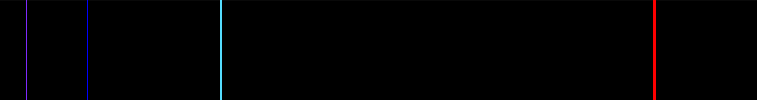
\includegraphics[width=0.7\textwidth]{graphics/Emission_spectrum-H.png}
    \label{fig:h_emit}
\end{figure}
By the end of the nineteenth century, a simple rule known as Balmer's formula (1885) showed how the frequencies of the different lines related to each other, though without explaining why this was, or making any prediction about the intensities. The formula also predicted some additional spectral lines in ultraviolet and infrared light that had not been observed at the time. These lines were later observed experimentally, raising confidence in the value of the formula. Balmer's formula states
\begin{linenomath}\begin{equation}
\frac1\lambda = R \left(\frac{1}{4}-\frac{1}{n^2}\right).
\end{equation}\end{linenomath}
In the present era, the $R$ for the atoms are called the Rydberg constant, which has the dimension $[L]^{-1};$ for hydrogen $R_H\simeq1.097\times10^7\,\mathrm{m}^{-1}.$ Rydberg showed in 1890 that the spectra of other elements could be organized by similar differences of \emph{terms}, and the Lyman, Paschen, Brackett, and Pfund series of hydrogen all take Balmer's form with the integer $4$ replaced by $1,9,16,25,\dots$

The decisive phenomenological principle was stated by Ritz in 1908. The \textbf{combination principle} asserts that every spectral line can be written as a difference of two spectral terms,
\begin{linenomath}
\begin{equation}
    \nu_{mn}=T_m-T_n,
\end{equation}
\end{linenomath}
so that the frequency of any line is determined by a pair of atomic levels, and new lines can be predicted as combinations of known ones. Spectroscopy thereby possessed, years before any theory, an exact algebra of its own: the observable quantities were not orbits or motions but pairs of states. Twenty years later this algebra of pairs would reappear as the multiplication rule of matrices (Section~\ref{subsec:matrix}).

The advantage of the term phenomenology was its completeness: a few dozen constants summarized thousands of lines, and the combination principle converted a chaos of frequencies into a table of levels. Its limitation was that the table cried out for a dynamical interpretation that classical physics could not supply. Why should an atom possess a discrete set of preferred energies at all?

\subsection{Bohr's Model of the Hydrogen Atom}
In 1913, H.~M.~Hansen asked Niels Bohr about Balmer's formula. Bohr recalled that ``As soon as I saw Balmer's formula, the whole thing was immediately clear to me.'' In \emph{On the Constitution of Atoms and Molecules}, he proposed a new model of the atom that included quantized electron orbits. This result is derived through the postulation of four hypotheses, listed as follows:
\begin{enumerate}
    \item The quantization of angular momentum, i.e., (orbit) angular momentum takes on a discrete set of values: $L = mvr = n\hbar.$ This implies the orbit of electrons is also discrete, instead of a continuum.
    \item The correspondence principle. The properties of the hydrogen atom should reduce to the classical results as $n\to \infty.$ As for a general system, this should hold as well insofar as all quantum numbers go to infinity.
    \item When an atom makes a transition from one stationary state to another, it emits or absorbs radiation whose frequency is given by the frequency condition $\omega = \frac{\Delta E}{\hbar}.$
    \item Apart from the angular momentum, any other generalized coordinate and momentum variables satisfy the condition (Bohr--Sommerfeld condition):\begin{linenomath}
        \begin{equation}
            \oint_{\text{over the phase curve}} p\dd q = n_qh.
        \end{equation}
    \end{linenomath}
\end{enumerate}
Bohr's calculation uses only circular orbits. Let us use not only circular orbits but also ellipsic ones so as to show the quantization of both angular and radial variables. The application of Hamilton-Jacobi equations is natural.

The action can be written
\begin{linenomath}
    \begin{equation}
        S=-Et+L\theta+\oint p_r\dd r.
    \end{equation}
\end{linenomath}
With $\partial S/\partial t=-E,$ $\partial S/\partial\theta=L,$ and $\partial S/\partial r=p_r,$ the Hamilton--Jacobi equation becomes
\begin{linenomath}
    \begin{equation}
        -E+\frac{p_r^{2}}{2m}+\frac{L^{2}}{2mr^{2}}-\frac{Ze^{2}}{r}=0,
    \end{equation}
\end{linenomath}
and solving for $p_r$ gives
\begin{linenomath}\begin{equation}
p_r = \sqrt{2mE-\frac{L^2}{r^2}+\frac{2mZe^2}{r}}.
\end{equation}\end{linenomath}
In the case of a constrained solution, the energy $E$ is typically negative. Therefore the equation above can be clarified as:
\begin{linenomath}\begin{equation}
p_r = \sqrt{-2m|E|-\frac{L^2}{r^2}+\frac{2mZe^2}{r}}.
\end{equation}\end{linenomath}
The radial action integral is evaluated by the substitution $u=1/r,$ which transforms the integrand into a form amenable to contour integration; the evaluation is cited without proof:\footnote{Under $u=1/r,$ $\dd r=-\dd u/u^{2},$ and the integral $\oint\sqrt{-A+B/r-C/r^{2}}\,\dd r$ with $A=2m|E|,$ $B=2mZe^{2},$ $C=L^{2}$ becomes $2\int_{u_{\min}}^{u_{\max}}\sqrt{-A+Bu-Cu^{2}}\,\dd u/u^{2}.$ Completing the square and evaluating by residues yields $2\pi(B/2\sqrt{A}-\sqrt{C}).$ The contour integration is a standard exercise in advanced classical mechanics; the steps are reproduced in textbooks on the old quantum theory (e.g., Born, \emph{The Mechanics of the Atom}, 1927).} The result is
\begin{linenomath}
    \begin{equation}
        \oint p_r\dd r = 2\int_{r_{\min{}}}^{r_{\max{}}} \sqrt{-2m|E|-\frac{L^2}{r^2}+\frac{2mZe^2}{r}} \dd r=2\pi\left( Ze^2\sqrt{\frac{m}{2|E|}}-L \right)=n_rh.
    \end{equation}
\end{linenomath}
Along with the quantization of angular momentum $L=n_\theta\hbar$ (from the angular action integral $\oint p_\theta\dd\theta=2\pi L=n_\theta h$), the radial condition gives
\begin{linenomath}
    \begin{equation}
        2\pi\Bigl(Ze^2\sqrt{\frac{m}{2|E|}}-n_\theta\hbar\Bigr)=n_r h=2\pi n_r\hbar,
    \end{equation}
\end{linenomath}
hence $Ze^2\sqrt{m/2|E|}=(n_r+n_\theta)\hbar=:n\hbar.$ Squaring and rearranging,
\begin{linenomath}
    \begin{align}
        \frac{Z^{2}e^{4}m}{2|E|}&=n^{2}\hbar^{2},
        &\quad|E|&=\frac{Z^{2}e^{4}m}{2n^{2}\hbar^{2}},
    \end{align}
\end{linenomath}
so that
\begin{linenomath}
    \begin{equation}
        E = -|E| = -\frac{Z^2e^4m}{2(n_r+n_\theta)^2\hbar^2}
        = -\frac{Z^2e^4m}{2n^2\hbar^2}.
    \end{equation}
\end{linenomath}
Therefore the energy level solely depends on the sum $n_r+n_\theta,$ which we denote by $n,$ and call by \textbf{principal quantum number}. A direct consequence of this result is the precise value of Rydberg's constant. By letting $n=2$ and $n,$ and thus by the emission frequency postulate one has
\begin{linenomath}
    \begin{equation}
        \frac{hc}{\lambda} = \frac{Z^2e^4m}{2\hbar^2}\left( \frac14-\frac{1}{n^2} \right).
    \end{equation}
\end{linenomath}
and so
\begin{linenomath}
    \begin{equation}
        \frac{1}{\lambda} = \frac{Z^2e^4m}{4\pi\hbar^3c}\left( \frac14-\frac{1}{n^2} \right),\quad R=\frac{Z^2e^4m}{4\pi\hbar^3c}.
    \end{equation}
\end{linenomath}
The result matches the experimental value very accurately.

The confirmations came quickly. The formula describes not only hydrogen but every one-electron ion; in particular the Pickering series, observed in stellar spectra in 1896 and long misattributed to hydrogen, follows at once for $Z=2$ and was thereby explained as ionized helium, with the small finite-nuclear-mass correction furnishing one of the most precise agreements in all of spectroscopy. In 1913--1914 Moseley measured the characteristic X-ray frequencies of the elements and found
\begin{linenomath}
    \begin{equation}
        \sqrt{\nu}\propto (Z-1),
    \end{equation}
\end{linenomath}
exactly as Bohr's model with $n=2\to1$ predicts; Moseley's law established the atomic number $Z,$ rather than the atomic weight, as the true ordering principle of the periodic table, and predicted the places of elements not yet discovered.

The advantage of Bohr's theory was not merely that it reproduced a known formula. It connected the Rydberg constant with the electron mass, charge, Planck's constant, and the Coulomb force. It also explained atomic stability in a provisional way: the electron did not spiral continuously into the nucleus because only certain stationary orbits were permitted. In this respect the theory was a remarkable bridge between classical mechanics and the quantum hypothesis.

But the bridge was visibly unfinished. The theory used classical orbits while forbidding most of them. It asserted stationary states without deriving why these states do not radiate. It assigned transition frequencies from energy differences, but did not describe the transition as a dynamical process. It succeeded brilliantly for hydrogen-like atoms, yet its extension to more complicated atoms required increasingly artificial rules. The theory therefore revealed both the power and the poverty of quantizing classical motion by hand.

\subsection{The Franck--Hertz Experiment}
Bohr's stationary states had been inferred from spectroscopy; the Franck--Hertz experiment of 1914 exhibited them in a collision. Franck and Hertz accelerated electrons through mercury vapor and measured the current reaching a collector. As the accelerating voltage is raised, the current rises until $4.9\,\mathrm{V},$ where it drops sharply; it rises again until $9.8\,\mathrm{V},$ drops again, and so on periodically. Electrons with less than $4.9\,\mathrm{eV}$ of kinetic energy cannot excite the mercury atom and pass through it elastically; electrons with more lose precisely $4.9\,\mathrm{eV}$ in a single inelastic collision, and the vapor simultaneously emits its ultraviolet resonance line at $253.7\,\mathrm{nm},$ whose photon energy is
\begin{linenomath}
    \begin{equation}
        h\nu=\frac{hc}{\lambda}=4.9\,\mathrm{eV}.
    \end{equation}
\end{linenomath}
An atom accepts energy from an electron beam only in the same discrete portions in which it emits light. (Franck and Hertz initially interpreted the $4.9\,\mathrm{V}$ threshold as an ionization potential; Bohr's reading of it as an excitation between stationary states was the historically decisive one.) The experiment earned Franck and Hertz the 1925 Nobel Prize.

The advantage of the Franck--Hertz experiment was its directness: stationary states were no longer an inference from line spectra but a fact of collision physics, measurable with a voltmeter. Its limitation was that it deepened the same mystery it confirmed. The atom evidently possessed discrete internal states of definite energy, yet nothing in the theory explained either their stability or the rule by which one state changed into another.

\subsection{The Bohr--Sommerfeld Theory}
Bohr's rules had been stated for the hydrogen atom. Their generalization to arbitrary separable mechanical systems was given independently by W.~Wilson in 1915 and by A.~Sommerfeld in 1915--1916: for every independent periodic degree of freedom of a multiply periodic system, the action integral over one cycle is an integer multiple of Planck's constant,
\begin{linenomath}
    \begin{equation}
        \oint p_i\,\dd q_i=n_i h
        \qquad (i=1,2,\dots,f).
    \end{equation}
\end{linenomath}
The hydrogen calculation of the previous section is precisely this machinery applied to the Kepler problem, and the two integers $n_r,n_\theta$ are its first fruits. Sommerfeld's systematic development, codified in his \emph{Atombau und Spektrallinien}, made three great additions.

First, elliptical orbits. With two quantum numbers the electron possesses a family of ellipses for each principal quantum number $n=n_r+n_\theta,$ and the energy's dependence on the sum alone --- the degeneracy --- is a peculiarity of the pure $1/r$ potential, rooted in the conservation of the Runge--Lenz vector.

Second, the relativistic fine structure. The velocity of the inner electron is a fraction $Z\alpha$ of $c,$ where
\begin{linenomath}
    \begin{equation}
        \alpha=\frac{e^2}{\hbar c}\simeq\frac{1}{137.04}
    \end{equation}
\end{linenomath}
is Sommerfeld's fine-structure constant, and the relativistic mass variation lifts the degeneracy:
\begin{linenomath}
    \begin{equation}
        E_{n,k}=-\frac{RhcZ^2}{n^2}\left[1+\frac{\alpha^2Z^2}{n}\left(\frac1k-\frac{3}{4n}\right)+\cdots\right],
        \qquad k=n_\theta=1,2,\dots,n.
    \end{equation}
\end{linenomath}
Paschen's precision measurements of the ionized-helium fine structure in 1916 agreed with this formula within experimental error, and the agreement was celebrated as the crown of the old quantum theory. Retrospectively the triumph was partly accidental: Sommerfeld's classical-relativistic formula coincides, for reasons no one at the time could have suspected, with the exact result of Dirac's relativistic electron theory, in which spin replaces the orbital quantum number in just the right way.

Third, space quantization. A third integer, $m,$ fixes the projection of the angular momentum on an external axis, so that the orientation of an orbit in space is itself quantized. The direct experimental display of this quantization came with the Stern--Gerlach experiment of 1922, whose full significance, however, belongs to a later section (Section~\ref{sec:twostate}). Finally, Ehrenfest's \emph{adiabatic principle} (1916) supplied the theory with its internal anchor: the quantities that remain invariant under slow variation of the external parameters are precisely the action integrals, and hence precisely the quantities that may be quantized. The old quantum theory thereby knew, in a precise sense, which of its rules were consistent.

The advantage of the Bohr--Sommerfeld theory was generality: it provided a uniform machinery --- classical mechanics plus action quantization plus correspondence arguments --- applicable to atoms, X-ray levels, the Stark and Zeeman effects, and molecular bands, and for one-electron systems it was quantitatively superb. Its limitation was that the machinery was a hybrid sewn onto classical dynamics rather than derived from anything deeper, and outside the separable, multiply periodic problems the seams split open at once.

\subsection{The Correspondence Principle}
The old quantum theory was not merely a list of numerical tricks. It was guided by a powerful requirement, the \textbf{correspondence principle}: quantum results must reproduce classical physics in the domain where classical physics is already known to work. For atomic systems this usually means the limit of large quantum numbers. In Bohr's language, the motion of an electron in a highly excited orbit should resemble the motion predicted by classical mechanics, and the radiation associated with transitions between nearby highly excited states should approach the classical orbital frequency.

The principle may be expressed schematically as follows. If $n$ is large and the transition is between neighboring levels, then
\begin{linenomath}
    \begin{equation}
        \nu_{n+1,n}=\frac{E_{n+1}-E_n}{h}
    \end{equation}
\end{linenomath}
should approach the characteristic frequency of the corresponding classical motion. The content of this statement is not that quantum theory is classically intuitive. Rather, it says that classical mechanics is a limiting description of a deeper theory. The old theory therefore had two obligations at once: it had to preserve classical mechanics where classical mechanics was successful, and it had to violate classical expectations where experiment required it.

Bohr and his school pressed the principle beyond frequencies into the territory the theory could not otherwise reach. Classically, the intensity and polarization of radiation are governed by the Fourier amplitudes of the orbital motion; by correspondence, the quantum transition probabilities between highly excited states should be governed by the same amplitudes, and selection rules should follow from the presence or absence of the relevant Fourier component. In Kramers's hands this program produced, in 1924--1925, a formula for the dispersion of light by atoms written entirely in terms of transitions between pairs of states --- the Kramers--Heisenberg formula --- in which the unobservable orbit had quietly been replaced by observable transition quantities. The bridge to the new mechanics was being built from the far side.

This principle remained essential in the transition to modern quantum mechanics. It helped determine which mathematical quantities in the new theory should correspond to position, momentum, energy, and angular momentum. But by itself it could not supply the new kinematics. It could say how the unknown theory must behave in a limit; it could not say what a quantum state is.

This is why the correspondence principle should be treated with care. Its advantage is methodological: it prevents quantum theory from becoming arbitrary by demanding contact with the classical world. It also preserves the genuine truth contained in classical mechanics. Its limitation is that it points backward as much as forward. It tells the new theory how to resemble the old theory when quantum numbers are large, but it does not explain what replaces an orbit, a trajectory, or a simultaneous assignment of position and momentum when quantum effects are essential.

\subsection{The Failures of the Old Quantum Theory}
The success of the Bohr--Sommerfeld theory should not be underestimated. It gave an astonishing account of the hydrogen spectrum and taught physicists that atomic stability and spectral discreteness were not accidental details to be repaired inside classical mechanics. Yet precisely because the theory was half classical and half quantum, its triumphs also revealed its limitations.

First, it retained the language of definite orbits while denying that all classical orbits were physically possible. The electron was still imagined as moving through a trajectory in space, but the permitted trajectories were selected by extra quantization rules. These rules were imposed from outside the classical equations; they were not consequences of the classical dynamics itself.

Second, the theory had no satisfactory account of quantum transitions. It could assign energies to stationary states and use the frequency condition
\begin{linenomath}
    \begin{equation}
        h\nu=E_i-E_f
    \end{equation}
\end{linenomath}
to predict emitted or absorbed radiation. But it did not explain what occurs during the transition, why a transition takes place, or how to compute its probability from first principles. Einstein's coefficients had shown that the transitions are genuinely chancy; the old theory could register the chance but not derive it.

Third, the old theory gave only a partial account of spectral intensities and selection rules. It could often locate spectral lines, but it could not generally explain why some lines are bright, some are weak, and some are absent. The actual data of spectroscopy are not only frequencies; they include probabilities, intensities, degeneracies, and rules of allowed transformation.

Fourth, the old theory did not generalize cleanly. Hydrogen-like atoms were its great triumph, but already helium, the next atom, defeated it: van Vleck's careful Bohr--Sommerfeld calculation of 1922 gave an ionization potential in plain disagreement with experiment, and no arrangement of quantized classical orbits could be made to work. The anomalous Zeeman effect was worse still, forcing Land\'e to introduce half-integer quantum numbers that made no sense within the whole-number machinery. Multi-electron atoms, molecular spectra, and magnetic effects revealed the poverty of the orbit picture. The later discovery of spin sharpened this difficulty: a two-valued degree of freedom appears in experiments without being reducible to a little classical rotation of a charged body.

Finally, wave-particle duality remained unresolved. Planck and Einstein had shown that radiation exchanges energy in quanta; de Broglie suggested that matter has wave-like character; interference phenomena continued to demand wave behavior. The old theory possessed pieces of the truth, but not the grammar in which those pieces could be spoken together.

The old quantum theory thus ended not with a refutation but with an accumulation of structural failures, all pointing the same way: the unobservable scaffolding of orbits had to go, and the observable algebra of transitions, already visible in Ritz's combination principle and in the Kramers--Heisenberg formula, had to become the foundation. This is precisely the point from which the modern theory departed.

\section{The Third Crisis: Waves, Particles, and Statistics}
By 1923 the quantum of energy was an established experimental fact, but its nature was more obscure than ever. Light interfered like a wave and recoiled like a particle; electrons were detected as particles and yet, it would soon appear, diffracted like waves; and the statistics by which quanta were counted turned out to be the statistics of no classical objects at all. The third crisis was therefore ontological: it concerned what kind of thing a quantum is. Its resolution required abandoning not merely this or that classical equation, but the classical division of the world into particles and waves altogether.

\subsection{The Compton Effect}
The single most persuasive experiment for the light quantum was performed by A.~H.~Compton in 1923. Compton scattered monochromatic X-rays from graphite and measured the wavelength of the scattered radiation as a function of angle. He found, beside an unshifted line, a shifted line whose wavelength increased with the scattering angle by exactly the amount predicted if the X-ray quantum collides with a single quasifree electron as one relativistic particle with another.

The kinematics is elementary. Let the incident and scattered photons have energies $h\nu,h\nu'$ and momenta $h\nu/c,h\nu'/c,$ and let the electron, initially at rest, recoil with momentum $\bm p.$ Conservation of energy and momentum reads
\begin{linenomath}
    \begin{equation}
        h\nu+mc^2=h\nu'+\sqrt{(pc)^2+m^2c^4},
        \qquad
        \bm p=\frac{h\nu}{c}\,\hat{\bm n}-\frac{h\nu'}{c}\,\hat{\bm n}',
    \end{equation}
\end{linenomath}
where $\theta$ is the angle between $\hat{\bm n}$ and $\hat{\bm n}'.$ Eliminating the electron variables,
\begin{linenomath}
    \begin{equation}
        p^2=\frac{h^2}{c^2}\left(\nu^2+\nu'^2-2\nu\nu'\cos\theta\right),
        \qquad
        \left[h(\nu-\nu')+mc^2\right]^2=p^2c^2+m^2c^4,
    \end{equation}
\end{linenomath}
Expanding the square on the left of the second equation,
\begin{linenomath}
    \begin{align}
        h^{2}(\nu-\nu')^{2}+2mc^{2}h(\nu-\nu')+m^{2}c^{4}=p^{2}c^{2}+m^{2}c^{4},
    \end{align}
\end{linenomath}
cancelling $m^{2}c^{4}$ and substituting $p^{2}c^{2}=h^{2}(\nu^{2}+\nu'^{2}-2\nu\nu'\cos\theta)$ from the first equation,
\begin{linenomath}
    \begin{align}
        h^{2}(\nu^{2}-2\nu\nu'+\nu'^{2})+2mc^{2}h(\nu-\nu')
        =h^{2}(\nu^{2}+\nu'^{2})-2h^{2}\nu\nu'\cos\theta.
    \end{align}
\end{linenomath}
Cancelling $h^{2}(\nu^{2}+\nu'^{2})$ from both sides,
\begin{linenomath}
    \begin{align}
        -2h^{2}\nu\nu'+2mc^{2}h(\nu-\nu')=-2h^{2}\nu\nu'\cos\theta,
    \end{align}
\end{linenomath}
which simplifies to
\begin{linenomath}
    \begin{equation}
        mc^2h(\nu-\nu')=h^2\nu\nu'(1-\cos\theta).
    \end{equation}
\end{linenomath}
To convert from frequency to wavelength, substitute $\nu=c/\lambda,$ $\nu'=c/\lambda',$ so that $\nu-\nu'=c(\lambda'-\lambda)/(\lambda\lambda')$ and $\nu\nu'=c^{2}/(\lambda\lambda').$ Then
\begin{linenomath}
    \begin{align}
        mc^{2}h\cdot\frac{c(\lambda'-\lambda)}{\lambda\lambda'}
        =h^{2}\cdot\frac{c^{2}}{\lambda\lambda'}\,(1-\cos\theta),
    \end{align}
\end{linenomath}
and cancelling the common factor $c^{2}h/(\lambda\lambda')$ yields the Compton formula
\begin{linenomath}
    \begin{equation}
        \Delta\lambda=\lambda'-\lambda=\frac{h}{mc}\,(1-\cos\theta),
        \qquad
        \frac{h}{m_ec}=2.43\times10^{-12}\,\mathrm{m}.
    \end{equation}
\end{linenomath}
The recoil electrons themselves were subsequently photographed in a cloud chamber by Compton and Simon, and their energies and directions were found to satisfy the same two-body kinematics. No wave theory of scattering can produce either the shift or the recoil.

The crisis can be measured by the remedies that serious physicists were willing to contemplate. In 1924 Bohr, Kramers, and Slater proposed to save the wave picture by sacrificing the exact conservation of energy and momentum in individual elementary processes, retaining them only statistically. Within a year the coincidence experiment of Bothe and Geiger had shown that in individual Compton events the scattered quantum and the recoil electron appear together, as strict conservation demands. Even the law of energy conservation had been put on trial, and the light quantum had survived it.

The advantage of the Compton effect was its finality: after 1923 the light quantum could no longer be described as a manner of speaking, for it possessed not only energy $h\nu$ but momentum $h\nu/c,$ and collided accordingly. Its limitation was that it made the wave-particle contradiction completely unavoidable. The same X-rays whose particle collisions Compton measured had been produced and monochromatized by Bragg diffraction --- a wave phenomenon --- in the very same apparatus.

\subsection{De Broglie's Matter Waves}
\label{subsec:debroglie}
The suggestion of de Broglie gave the old quantum theory one of its most suggestive interpretations. If light, formerly understood as a wave, also behaves as a particle in energy exchange, perhaps matter, formerly understood as particles, also possesses a wave-like character. De Broglie's argument of 1924 was guided by relativity: a particle of rest mass $m_0$ carries in its rest frame an internal oscillation of frequency $m_0c^2/h,$ and the demand that this oscillation remain in phase with a wave of frequency $E/h$ in every frame --- the ``harmony of phases'' --- fixes the wave's dispersion uniquely. The proposed relation
\begin{linenomath}
    \begin{equation}
        \lambda=\frac{h}{p}
    \end{equation}
\end{linenomath}
turns Bohr's angular momentum rule into a standing-wave condition. For a circular orbit,
\begin{linenomath}
    \begin{equation}
        2\pi r=n\lambda
    \end{equation}
\end{linenomath}
is equivalent, via $\lambda=h/p=h/mv,$ to
\begin{linenomath}
    \begin{equation}
        2\pi r=n\frac{h}{mv}\quad\Longrightarrow\quad mvr=n\frac{h}{2\pi}=n\hbar.
    \end{equation}
\end{linenomath}
What had looked like an arbitrary restriction on orbits could now be read as the condition that the electron wave fit consistently around the orbit.

This was an immense conceptual advantage. Quantization no longer appeared merely as an imposed arithmetic rule; it resembled the discreteness of normal modes in acoustics or optics. But the limitation remained: if the electron is a wave, what physical quantity does the wave represent? It cannot be simply an ordinary material density, for electrons are detected as localized events. Nor can it be an ordinary classical probability distribution, because probabilities do not interfere with one another. The matter-wave idea therefore brought the theory closer to the modern language of amplitudes, but it did not by itself provide the interpretation of those amplitudes.

The experimental verdict was delivered by diffraction. Elsasser pointed out in 1925 that a crystal grating should diffract slow electrons if de Broglie was right. In 1927 Davisson and Germer, studying the scattering of electrons from a nickel single crystal, found a pronounced reflection maximum at precisely the angle and energy predicted by $\lambda=h/p$ with the crystal's known spacing; independently, G.~P.~Thomson passed electrons through thin metallic foils and obtained the ring patterns characteristic of wave diffraction by a polycrystal.\footnote{History here permitted itself a small irony: J.~J.~Thomson received the Nobel Prize for showing that the electron is a particle, and his son G.~P.~Thomson received it (with Davisson, 1937) for showing that the electron is a wave.} De Broglie received the 1929 Nobel Prize. Matter waves were no longer a hypothesis but a measurement.

\subsection{Bose, Einstein, and the Statistics of Quanta}
In June 1924 Einstein received from Dacca a short paper by an unknown lecturer, S.~N.~Bose, with a request for help in publication. Bose had derived Planck's law without any appeal to electromagnetism at all. Treat the radiation in a cavity as a gas of light quanta; divide the one-particle phase space into cells of volume $h^3,$ so that the frequency interval $(\nu,\nu+\dd\nu)$ contains
\begin{linenomath}
    \begin{equation}
        A_s=\frac{8\pi\nu_s^2V}{c^3}\,\dd\nu_s
    \end{equation}
\end{linenomath}
cells (the factor two being the two polarizations); and count, as Boltzmann taught, the number of ways of realizing each distribution of quanta among cells. Bose's decisive step was to count the cells as distinguishable but the quanta as indistinguishable: what matters is only how many quanta occupy each cell, never which ones. The number of complexions is then
\begin{linenomath}
    \begin{equation}
        W=\prod_s\frac{(A_s+N_s-1)!}{N_s!\,(A_s-1)!},
    \end{equation}
\end{linenomath}
and maximizing the entropy $k_B\log W$ at fixed total energy yields the equilibrium distribution. Applying Stirling's approximation $\log n!\simeq n\log n-n$ to each factor, and ignoring unity against large $A_s,N_s,$
\begin{linenomath}
    \begin{align}
        \log W\simeq\sum_{s}\bigl[(A_s+N_s)\log(A_s+N_s)-N_s\log N_s-A_s\log A_s\bigr].
    \end{align}
\end{linenomath}
Maximizing $S=k_B\log W$ with respect to the occupation numbers $N_s,$ subject to the constraint $\sum_s N_s h\nu_s=E$ (fixed total energy), introduces a single Lagrange multiplier $\beta$:
\begin{linenomath}
    \begin{align}
        \frac{\partial}{\partial N_s}\bigl(\log W-\beta\sum_{r}N_r h\nu_r\bigr)=0
        \;\Longrightarrow\;
        \log\frac{A_s+N_s}{N_s}-\beta h\nu_s=0,
    \end{align}
\end{linenomath}
hence $(A_s+N_s)/N_s=e^{\beta h\nu_s},$ and the mean occupation per cell is
\begin{linenomath}
    \begin{equation}
        \frac{\bar N_s}{A_s}=\frac{1}{e^{\beta h\nu_s}-1}.
    \end{equation}
\end{linenomath}
The thermodynamic definition of temperature, $\partial S/\partial E=1/T,$ identifies $\beta=1/k_BT;$ the identification is cited without proof from equilibrium thermodynamics.\footnote{In a rigorous treatment, $\beta=1/k_BT$ follows from the definition $1/T=\partial S/\partial E.$ The absence of a number-conservation Lagrange multiplier (chemical potential) reflects the fact that photons are freely created and absorbed at the cavity walls, so the photon number is not independently conserved.} The result is the Planck mean occupation,
\begin{linenomath}
    \begin{equation}
        \frac{\bar N_s}{A_s}=\frac{1}{e^{h\nu_s/k_BT}-1},
    \end{equation}
\end{linenomath}
which is Planck's law. Einstein recognized the derivation's importance at once, translated the paper himself, and saw it into print.

Einstein then did something Bose had not attempted: he applied the same counting to an ideal gas of material particles. The result was a new statistics --- \textbf{Bose--Einstein statistics} --- differing from Boltzmann's at low temperature, where the gas exhibits a phase transition of an entirely new kind, the \textbf{Bose--Einstein condensation}, in which a finite fraction of the particles accumulates in the single lowest state.\footnote{The condensation was observed directly only in 1995, in dilute gases of alkali atoms at microkelvin temperatures, seventy years after its prediction.} Two years later Fermi and Dirac completed the picture with the statistics obeyed by particles subject to Pauli's exclusion principle. That integer-spin particles obey Bose--Einstein statistics and half-integer-spin particles Fermi--Dirac statistics --- the spin-statistics theorem --- was proved by Pauli in 1940 within relativistic quantum field theory.

The advantage of Bose's counting was that it made the particle picture of light self-consistent for the first time: Planck's law followed from quanta alone, without waves, provided the quanta were counted as indistinguishable. Its limitation was profound and pregnant: indistinguishability is not a property of any classical objects. Classical particles can always be labeled by their trajectories. The new statistics was an early, quantitative sign that a quantum is neither a classical particle nor a classical wave, but something for which classical language has no ready category --- a sign that the later formalism would honor by representing states as vectors in a space where permutations act trivially (see the chapter on second quantization).

\subsection{The Exclusion Principle and Electron Spin}
\label{subsec:spin}
The last discoveries of the old period were forced by the spectroscopy of many-electron atoms. Pauli's analysis of the alkali spectra and the anomalous Zeeman effect convinced him, in 1925, that the electron requires a fourth quantum number capable of only two values --- in his phrase, a ``classically non-describable two-valuedness'' --- and that no two electrons in an atom may agree in all four quantum numbers. This \textbf{exclusion principle} explained at one stroke the closing of the electron shells and hence the structure of the periodic table, which the orbit theory had never been able to derive.

Later the same year Uhlenbeck and Goudsmit identified the two-valued degree of freedom with an intrinsic angular momentum: the electron carries a spin of magnitude $\hbar/2$ and a magnetic moment twice as large as classical electromagnetism would assign to a rotating charge.\footnote{The idea had occurred earlier to Kronig, who discussed it with Pauli and was so thoroughly discouraged by him that he never published; Uhlenbeck and Goudsmit's manuscript was nearly withdrawn for the same reason, and survived because Ehrenfest had already sent it to the journal.} The factor of two --- the anomalous gyromagnetic ratio --- was precisely what the anomalous Zeeman patterns required, and Thomas's relativistic precession of 1926 repaired the one remaining discrepancy in the fine structure. The Stern--Gerlach experiment of 1922, which had sent a beam of silver atoms through an inhomogeneous magnetic field and observed two discrete spots instead of a continuous smear, could now be read as the direct display of the two spin orientations of the valence electron; its modern analysis occupies Section~\ref{sec:twostate}.

The advantage of the spin hypothesis was enormous: it closed the periodic table, explained the Zeeman patterns, and gave the two-valuedness a definite mechanical content. Its limitation was equally significant for everything that follows. Spin-$\tfrac12$ is a physical observable taking exactly two values, with no continuous classical analogue; no model of a rotating body reproduces its properties, and the attempt to picture it classically fails quantitatively by the factor of two. Here, inside the atom itself, experiment had produced the simplest possible quantum system: two alternatives, and nothing in between.

\section{The Birth of Modern Quantum Mechanics}
By the middle of the 1920s, the old quantum theory had become both indispensable and unsatisfactory. Its successes showed that quantization was not a passing curiosity; its failures showed that quantization could not remain a set of external restrictions imposed on classical motion. The decisive change came when physicists stopped asking how to choose the allowed classical orbits and began asking what should replace the classical description of motion itself.

Two formulations appeared almost simultaneously. Heisenberg's matrix mechanics began from observable transition data and abandoned electron orbits. Schrodinger's wave mechanics began from de Broglie's matter waves and recast bound states as eigenvalue problems. At first these theories looked very different, almost opposed in spirit: one algebraic and discontinuous, the other analytic and wave-like. Their eventual equivalence revealed one of the deepest lessons of quantum mechanics: the representation is not the physical essence. A quantum state can be represented by a column of coefficients, a wave function, or another set of coordinates adapted to the experiment.

\subsection{Heisenberg and the Abandonment of Orbits}
\label{subsec:matrix}
Heisenberg's 1925 work began from a radical act of discipline. If electron orbits inside atoms are not observable, then perhaps the theory should not use them as fundamental objects. Spectroscopy gives transition frequencies and intensities. These quantities naturally carry two labels: an initial stationary state and a final stationary state. Instead of a classical quantity $x(t)$ along an orbit, one considers an array of transition quantities
\begin{linenomath}
    \begin{equation}
        x_{mn},
    \end{equation}
\end{linenomath}
where $m$ and $n$ label stationary states.

The time dependence associated with a transition is governed by Bohr's frequency condition:
\begin{linenomath}
    \begin{equation}
        x_{mn}(t)=x_{mn}\exp\left(2\pi i\nu_{mn}t\right),
        \qquad
        h\nu_{mn}=E_m-E_n.
    \end{equation}
\end{linenomath}
The multiplication rule for such quantities is not arbitrary. It is inherited from the way Fourier components combine in classical mechanics, but with a decisive change of labels. For a classical periodic motion one may write
\begin{linenomath}
    \begin{equation}
        x(t)=\sum_{\alpha}x_{\alpha}\exp(2\pi i\nu_{\alpha}t),
        \qquad
        y(t)=\sum_{\beta}y_{\beta}\exp(2\pi i\nu_{\beta}t).
    \end{equation}
\end{linenomath}
The product $x(t)y(t)$ has components obtained by convolution, because frequencies add:
\begin{linenomath}
    \begin{equation}
        (xy)_{\gamma}
        =
        \sum_{\alpha+\beta=\gamma}x_{\alpha}y_{\beta}.
    \end{equation}
\end{linenomath}
In spectroscopy, however, the relevant frequency is not attached to a single orbit harmonic but to a pair of energy levels. The Ritz combination principle gives
\begin{linenomath}
    \begin{equation}
        \nu_{mk}+\nu_{kn}
        =
        \frac{E_m-E_k}{h}+\frac{E_k-E_n}{h}
        =
        \nu_{mn}.
    \end{equation}
\end{linenomath}
Thus the analogue of adding Fourier frequencies is composing transitions through an intermediate state. If a transition from $m$ to $n$ can pass through intermediate states $k,$ then the product of two quantities has components
\begin{linenomath}
    \begin{equation}
        (AB)_{mn}=\sum_k A_{mk}B_{kn}.
    \end{equation}
\end{linenomath}
Born recognized this rule as matrix multiplication. The noncommutativity is now easy to understand: $AB$ sums over paths in which $B$ acts first and $A$ acts second, while $BA$ sums over the reversed order. Since the intermediate amplitudes need not be the same, the crucial consequence is that, in general,
\begin{linenomath}
    \begin{equation}
        AB\neq BA.
    \end{equation}
\end{linenomath}
Thus noncommutativity entered quantum mechanics not as an ornament of later formalism, but as a structural replacement for classical kinematics.

Born and Jordan, and soon Dirac, developed this into a mechanics of noncommuting quantities. The canonical variables satisfy
\begin{linenomath}
    \begin{equation}
        QP-PQ=i\hbar I.
    \end{equation}
\end{linenomath}
Historically, this relation was also guided by the correspondence principle. In classical Hamiltonian mechanics, the Poisson bracket of position and momentum is
\begin{linenomath}
    \begin{equation}
        \{q,p\}=1.
    \end{equation}
\end{linenomath}
Dirac observed that the quantum commutator plays the role of the Poisson bracket multiplied by $i\hbar$:
\begin{linenomath}
    \begin{equation}
        \{A,B\}
        \quad\longrightarrow\quad
        \frac{1}{i\hbar}[A,B],
        \qquad
        [A,B]=AB-BA.
    \end{equation}
\end{linenomath}
Applied to $q$ and $p,$ this rule gives $[Q,P]=i\hbar I.$ This is not a proof in the Euclidean sense; it is a correspondence deduction, tying the new algebra to the old mechanics in the limit where actions are large compared with $\hbar.$ The relation has no analogue in classical multiplication, where position and momentum are ordinary functions on phase space and therefore commute. It says that the order of operations matters. The old orbit in phase space is replaced by an algebra of possible transformations and measurements.

The new mechanics proved itself almost immediately. In January 1926 Pauli solved the hydrogen atom purely within matrix mechanics, exploiting the Runge--Lenz vector as a matrix constant of motion, and recovered the Balmer spectrum without a single wave or differential equation. The austere algebra could do everything the orbit picture could do, and it could do things the orbit picture could not.

The advantage of matrix mechanics was its faithfulness to spectroscopic data. It dealt directly with transition frequencies, intensities, and selection rules, precisely where the old theory had been weakest. It also naturally described discrete spectra. Its limitation was its initial opacity. It did not offer an intuitive picture of an electron moving in space, nor did it immediately explain why a familiar-looking differential equation should emerge for particles in potentials. It was a powerful algebraic grammar, but at first it seemed physically austere.

\subsection{Schrodinger's Wave Mechanics}
Schrodinger's route was quite different. Inspired by de Broglie's matter waves and by Hamilton's optical analogy, he sought an equation whose stationary solutions would give the allowed states of an electron. Hamilton had already observed in the 1830s that the equations of mechanics in action form are formally identical to the equations of geometrical optics in eikonal form: a system of trajectories resembles a system of rays. If matter possesses a wave nature, then classical mechanics should stand to some deeper wave mechanics as geometrical optics stands to wave optics --- valid when the wavelength is negligible, and powerless to explain diffraction. Schrodinger's program was to write down the wave equation of which classical mechanics is the short-wavelength limit. In the nonrelativistic case, the central equation became
\begin{linenomath}
    \begin{equation}
        i\hbar\frac{\partial \psi}{\partial t}
        =
        \left(-\frac{\hbar^2}{2m}\nabla^2+V\right)\psi.
    \end{equation}
\end{linenomath}
One quick deduction of its form begins from a free matter wave
\begin{linenomath}
    \begin{equation}
        \psi(x,t)
        =
        \exp\left[\frac{i}{\hbar}(p\cdot x-Et)\right].
    \end{equation}
\end{linenomath}
For this wave,
\begin{linenomath}
    \begin{equation}
        -i\hbar\nabla\psi=p\psi,
        \qquad
        i\hbar\frac{\partial\psi}{\partial t}=E\psi.
    \end{equation}
\end{linenomath}
The classical nonrelativistic energy relation is
\begin{linenomath}
    \begin{equation}
        E=\frac{p^2}{2m}+V(x).
    \end{equation}
\end{linenomath}
Replacing $E$ and $p$ by the differential operations that reproduce their eigenvalues on plane waves,
\begin{linenomath}
    \begin{equation}
        E\mapsto i\hbar\frac{\partial}{\partial t},
        \qquad
        p\mapsto -i\hbar\nabla,
    \end{equation}
\end{linenomath}
gives Schrodinger's equation. Again, this is not a derivation from classical mechanics alone. It is a controlled guess: de Broglie's wave relations supply the phase, the classical energy relation supplies the dispersion, and the correspondence principle tells us how to translate energy and momentum into operations on amplitudes.

For states of definite energy, one writes
\begin{linenomath}
    \begin{equation}
        \psi(x,t)=\phi(x)\exp\left(-\frac{iEt}{\hbar}\right),
    \end{equation}
\end{linenomath}
and obtains the time-independent equation
\begin{linenomath}
    \begin{equation}
        \left(-\frac{\hbar^2}{2m}\nabla^2+V\right)\phi=E\phi.
    \end{equation}
\end{linenomath}
The allowed energies are therefore eigenvalues of a differential operator.

This was mathematically and physically illuminating. The discreteness of bound-state energies no longer had to be imposed through Bohr-Sommerfeld integrals; it could arise from boundary conditions on wave functions. A bound electron resembles a standing wave, and the hydrogen atom can be treated without literal electron orbits. In a celebrated series of four communications of 1926, \emph{Quantisierung als Eigenwertproblem}, Schrodinger solved the hydrogen atom, the harmonic oscillator, and the rigid rotor, developed perturbation theory, and computed the Stark effect. In this sense wave mechanics preserved something intuitive from classical physics: differential equations, spatial functions, and analogies with optics.

Yet the same intuitive strength concealed a danger. Schrodinger initially hoped that the wave might be a real charge distribution. But localized detections, scattering events, and the individuality of particles resisted this interpretation. A wave spread through space does not look like a point-like detection on a screen. Thus wave mechanics had a clear mathematical form before it had a clear physical interpretation.

\subsection{Born's Probability Interpretation}
\label{subsec:born-probability}
Born's interpretation supplied the missing bridge. In his scattering papers of 1926, Born argued that the wave function of a scattered particle should not be read as a material density but as a probability amplitude: the wave determines not where the particle is, but where it is likely to be found.\footnote{The interpretation appeared first in a footnote of Born's preliminary communication, in which the probability of a scattering direction is taken proportional to the squared modulus of the corresponding wave amplitude. Born had to wait until 1954 for the Nobel Prize awarded for this step.} For a normalized wave function, the probability of finding the particle in a spatial region $\Omega$ is
\begin{linenomath}
    \begin{equation}
        \int_{\mathbb{R}^3}|\psi(x)|^2\,\dd^3x=1,
        \qquad
        P(\Omega)=\int_{\Omega}|\psi(x)|^2\,\dd^3x.
    \end{equation}
\end{linenomath}
Thus $\psi$ itself is not a directly observable quantity. Its modulus squared gives probabilities, while its phase can influence later probabilities through interference.

The compatibility of this interpretation with Schrodinger's equation can be checked directly. Let
\begin{linenomath}
    \begin{equation}
        \rho(x,t)=|\psi(x,t)|^2.
    \end{equation}
\end{linenomath}
Using Schrodinger's equation and its complex conjugate, one obtains the continuity equation
\begin{linenomath}
    \begin{align}
        \frac{\partial\rho}{\partial t}
        &= \psi^{*}\frac{\partial\psi}{\partial t} + \frac{\partial\psi^{*}}{\partial t}\psi
         = \psi^{*}\Bigl(\frac{i\hbar}{2m}\nabla^{2}\psi - \frac{i}{\hbar}V\psi\Bigr)
           + \Bigl(-\frac{i\hbar}{2m}\nabla^{2}\psi^{*} + \frac{i}{\hbar}V\psi^{*}\Bigr)\psi
           \nonumber\\
        &= \frac{i\hbar}{2m}\bigl(\psi^{*}\nabla^{2}\psi - \psi\nabla^{2}\psi^{*}\bigr)
         = -\nabla\cdot\Bigl[\frac{\hbar}{2mi}\bigl(\psi^{*}\nabla\psi - \psi\nabla\psi^{*}\bigr)\Bigr]
         =: -\nabla\cdot\bm j,
    \end{align}
\end{linenomath}
where the third equality uses $\psi^{*}\nabla^{2}\psi-\psi\nabla^{2}\psi^{*}
=\nabla\cdot(\psi^{*}\nabla\psi-\psi\nabla\psi^{*})$,
giving the probability current
\begin{linenomath}
    \begin{equation}
        \bm j = \frac{\hbar}{2mi}\bigl(\psi^{*}\nabla\psi - \psi\nabla\psi^{*}\bigr).
    \end{equation}
\end{linenomath}
Integrating over all space, and assuming the wave function vanishes sufficiently fast at infinity, gives
\begin{linenomath}
    \begin{equation}
        \frac{\dd}{\dd t}\int_{\mathbb{R}^3}|\psi(x,t)|^2\,\dd^3x=0.
    \end{equation}
\end{linenomath}
Thus the squared norm is conserved by the dynamics. This is a major advantage of the wave equation as a probability-amplitude equation: it preserves the total probability without an additional postulate.

This interpretation transformed the meaning of the wave equation. The wave function is not a classical wave of matter in the same sense that a water wave is a wave of water. It is a complex amplitude encoding the statistical predictions of a preparation. The advantage of Born's rule is that it explains why wave mechanics can produce localized experimental outcomes while retaining interference. Its limitation is conceptual: it makes probability fundamental in a way foreign to classical mechanics. The theory predicts distributions of outcomes, not hidden trajectories of the old kind. The ``chance'' that Einstein had been forced to admit in his theory of radiation had become irreducible.

\subsection{The Equivalence of the Two Pictures}
\label{subsec:equivalence}
The relation between matrix mechanics and wave mechanics was clarified by Schrodinger, Dirac, and others. A wave function can be expanded in a basis of stationary states:
\begin{linenomath}
    \begin{equation}
        \psi(x)=\sum_n c_n\phi_n(x).
    \end{equation}
\end{linenomath}
If the basis is orthonormal, then
\begin{linenomath}
    \begin{equation}
        \int \phi_m^*(x)\phi_n(x)\,\dd^3x=\delta_{mn},
        \qquad
        c_n=\int \phi_n^*(x)\psi(x)\,\dd^3x.
    \end{equation}
\end{linenomath}
In this representation, the state is described by the coefficients $c_n.$ Operators acting on wave functions acquire matrix elements
\begin{linenomath}
    \begin{equation}
        A_{mn}=\int \phi_m^*(x)\,A\,\phi_n(x)\,\dd^3x.
    \end{equation}
\end{linenomath}
Indeed, if
\begin{linenomath}
    \begin{equation}
        (A\psi)(x)=\sum_m d_m\phi_m(x),
    \end{equation}
\end{linenomath}
then
\begin{linenomath}
    \begin{equation}
        d_m=\sum_n A_{mn}c_n.
    \end{equation}
\end{linenomath}
The differential operator has become a matrix acting on the coefficient column. In the same way, Schrodinger's equation becomes
\begin{linenomath}
    \begin{equation}
        i\hbar\dot c_m=\sum_n H_{mn}c_n.
    \end{equation}
\end{linenomath}
Thus the matrix and wave pictures are not rival descriptions of different worlds. They are different representations of the same abstract structure.

This equivalence is historically decisive for the present notes. It suggests that the physical state should not be identified too quickly with any one representation, whether an orbit, a matrix column, or a wave function in space. What is invariant is the network of transition amplitudes, probabilities, and transformations. The language of Hilbert space is the mathematical distillation of this insight: states are vectors up to phase, measurable alternatives correspond to decompositions into basis vectors, and physical transformations act linearly on amplitudes.

The modern theory therefore did not arise by simply choosing a more complicated equation of motion. It arose by replacing the classical kinematics of points in phase space with a kinematics of states, amplitudes, and noncommuting transformations. It remained to give this one theory its final, representation-independent form.

\subsection{Dirac, Jordan, and von Neumann: the General Formalism}
\label{subsec:djv-formalism}
The synthesis was completed in a remarkably short time. Dirac and Jordan, independently in 1926--1927, formulated the \textbf{transformation theory}: the physical content of the theory lies in the transition amplitudes between the eigenstates of arbitrary observables, and the wave function and the matrix column are merely two coordinate systems for one and the same abstract vector. To handle observables with continuous spectra, Dirac introduced the $\delta$ function; his \emph{Principles of Quantum Mechanics} of 1930 presented the whole theory in the language of kets, bras, and operators that this note also uses.\footnote{Dirac's bra-ket notation itself was introduced in a paper of 1939; the 1930 book still wrote the inner product in the older form $(\psi,\phi)$.}

Von Neumann then gave the theory its rigorous mathematical foundation. In papers of 1927 and definitively in his \emph{Mathematische Grundlagen der Quantenmechanik} of 1932, he identified the arena of quantum states as the abstract Hilbert space, observables as self-adjoint operators upon it, measurable spectra as their spectra in the sense of functional analysis, and statistical predictions as the trace rule $\langle A\rangle=\tr(\rho A).$ In the same years Heisenberg's uncertainty relation (1927) exhibited the quantitative limit on the joint determination of canonically conjugate quantities, and Bohr's doctrine of complementarity, announced at Como in September 1927, gave the conceptual frame in which mutually exclusive experimental arrangements complete rather than contradict one another; both themes are developed systematically in the chapter on measurement. Wigner and Weyl brought the theory of group representations into quantum mechanics, preparing the modern understanding of symmetry that a later chapter will develop. The fifth Solvay Congress of 1927, devoted to ``Electrons and Photons,'' is conventionally taken as the closing scene of the founding period and the opening of the Einstein--Bohr debate on its meaning.

The advantage of the Dirac--Jordan--von Neumann formulation was its completeness and its generality: one theory, representation-independent, mathematically precise, embracing the matrix and wave pictures as special cases and finite-dimensional spin systems and infinite-dimensional scattering systems alike. Its limitation was of a different order from all the limitations recorded above. The formalism was finished before its interpretation was settled; what a measurement is, and what the state vector knows, remained --- and in part remains --- an open question. But the question could now be stated precisely, and these notes will take it up with the same precision.

\subsection{Why a New Kinematics Was Needed}
\label{subsec:why-kinematics}
Looking back over the three crises, one can locate the exact point at which classical physics broke. It was not a force law that failed, nor any particular equation of motion. What failed was the concept of \emph{state} itself, and with it the concept of a measurable quantity. A failure of this kind is called \textbf{kinematical}, in distinction from a dynamical one: kinematics fixes what kind of object a state is and what questions may be asked of it, while dynamics merely says how the state evolves in time. The kinematics of classical mechanics is quickly stated. The state of a particle is a point of phase space --- a simultaneous assignment of position and momentum; an observable is a function on phase space; and the result of a measurement is, in principle, nothing but the value of that function, possessed by the system before and after the measurement alike.

Against this scheme, each crisis of the old quantum theory contributed one precise objection, and the modern theory may be read as the minimal kinematics answering all of them at once.

First, the radiation crisis and the specific heats showed that the energies available to a bounded microscopic system may form a discrete set. The state of such a system is therefore not an arbitrary point of a continuum: it is one of a discrete list of experimentally distinguishable alternatives --- the stationary states of Bohr, exhibited directly in the collisions of Franck and Hertz.

Second, the combination principle of Ritz showed that the observable data of atomic physics are attached not to single states but to \emph{pairs} of states: a spectral line lives on a transition. Physical quantities are therefore not numbers possessed by a state, but relations between two states --- the form in which Heisenberg received them when he built matrix mechanics.

Third, the interference of light and of matter showed that alternatives do not combine as probabilities do. Two open paths can produce fewer counts at a detector than one. The quantities that add must therefore be capable of cancelling: they are complex \emph{amplitudes}, and the probabilities are their squared moduli. Born's rule, read backward from experiment, is the statement that nature composes alternatives by amplitudes and interrogates them by probabilities.

Fourth, the commutator $[Q,P]=i\hbar I$ showed that the order of physical operations matters. If two observables multiplied in different orders give different results, then no state can assign sharp pre-existing values to both, and the classical picture of the state as a complete catalogue of properties is untenable in principle rather than merely in practice.

Fifth, the equivalence of the matrix and wave mechanics showed that the state itself is none of its representations: not the orbit, not the wave function, not the column of coefficients, but that which is common to all of them --- an abstract object to which every experimental basis assigns its own list of amplitudes.

A kinematics meeting these five requirements must therefore provide: for every experiment a set of mutually exclusive alternatives; complex amplitudes for the transitions between preparations and outcomes; probabilities as squared moduli of amplitudes; a noncommutative composition of operations; and a notion of state independent of the basis in which it is described. This is precisely the Hilbert-space kinematics of Dirac and von Neumann, whose systematic construction occupies the next chapter. Before that construction, it is worth seeing the five requirements at work in the simplest possible arena, where each of them can be traced back to a definite experiment.

\subsection*{A Synoptic Chronology}
For convenience, the principal events of the chapter are collected below.
\begin{table}[htbp!]
    \centering
    \caption{A synoptic chronology of the developments described in this chapter.}
    \begin{tabular}{ll}
        \toprule
        Year & Event \\
        \midrule
        1801--03 & Young: the interference of light \\
        1809 & Malus: polarization by reflection; the cosine-squared law \\
        1859--60 & Kirchhoff: universality of the black-body spectrum \\
        1879--84 & Stefan's law; Boltzmann's thermodynamic derivation \\
        1885--90 & Balmer's formula; Rydberg's term analysis \\
        1891--92 & Zehnder and Mach: the interferometer \\
        1893--96 & Wien's displacement law and exponential spectrum \\
        1897 & Thomson: the electron \\
        1900 & Rubens--Kurlbaum; Planck's formula and the quantum of action \\
        1905 & Einstein: the light quantum; Jeans completes Rayleigh's law \\
        1907 & Einstein: the specific heat of solids \\
        1908 & Ritz's combination principle \\
        1909 & Taylor: interference at feeble light \\
        1909--11 & Geiger--Marsden scattering; Rutherford's nucleus; first Solvay Congress \\
        1913--14 & Bohr's atom; Moseley's law; Franck--Hertz experiment \\
        1915--16 & Wilson--Sommerfeld quantization; relativistic fine structure \\
        1916--17 & Einstein's $A$ and $B$ coefficients \\
        1922 & Stern--Gerlach experiment \\
        1923 & Compton effect \\
        1924 & Bose's counting; de Broglie's thesis; Bohr--Kramers--Slater theory \\
        1925 & Bothe--Geiger refutes BKS; Pauli exclusion; electron spin; \\
               & Heisenberg's mechanics; Born--Jordan and Dirac complete it \\
        1926 & Schrodinger's four papers; Born's probability rule; equivalence; \\
               & Fermi--Dirac statistics \\
        1927 & Davisson--Germer and G.~P.~Thomson; uncertainty; complementarity; \\
               & Dirac--Jordan transformation theory; fifth Solvay Congress \\
        1930--32 & Dirac's \emph{Principles}; von Neumann's \emph{Foundations} \\
        \bottomrule
    \end{tabular}
\end{table}

\section{Two-State Experiments and the Language of Amplitudes}
\label{sec:twostate}
The kinematics sketched above was distilled by its founders from the whole of atomic physics, but its content is already fully visible in experiments so simple that the apparatus can return only one of two answers: this detector or that one, transmitted or absorbed, upper spot or lower spot. A system interrogated by such an experiment is called, relative to that experiment, a \textbf{two-state system}. Two-state systems are not a modern invention. Three families of them have already crossed this narrative: interference between two optical paths, known since Young's double-slit experiments and sharpened into the interferometers of Zehnder and Mach in the 1890s; polarization, whose cosine-squared law Malus discovered in 1809; and the two spots of Stern and Gerlach's silver beam of 1922. After 1927 these old devices were revisited with single quanta, one at a time, and each was found to exhibit precisely the requirements of the preceding section: alternatives that combine by amplitudes, probabilities that depend on the basis of the question, measurements that prepare rather than merely reveal.

The notation in which these experiments are now described is Dirac's, devised for the transformation theory. An experimentally distinguishable alternative is written as a ket, as in $\ket{u}$ or $\ket{+z};$ the superposition of alternatives is written as a linear combination of kets; the amplitude for a system prepared in the alternative $\ket{\psi}$ to be found in the alternative $\ket{\phi}$ is written $\braket{\phi|\psi};$ and the probability of that transition is $|\braket{\phi|\psi}|^2.$ These conventions merely transcribe Born's rule and the superposition of amplitudes into a compact script. The experiments of this section show why no simpler script is sufficient. The advantage of beginning with two-state systems is that every essential novelty appears without the analytic machinery of wave equations on continuous space; the limitation is equally clear, for real particles move in space, carry momentum, and may possess infinitely many alternatives. The two-state examples show the grammar in its simplest sentence, not the whole language.

\subsection{The Interference of Single Quanta}
Interference was, historically, the fortress of the wave theory of light: the fringes of Young's double-slit experiments of 1801--1803 were its founding evidence. The fortress was tested at its weakest point by G.~I.~Taylor in 1909. Photographing the shadow of a needle in light so feeble that, on the quantum hypothesis, only one light quantum at a time could be present in the apparatus, he found after exposures lasting up to three months that the interference fringes were entirely unchanged. The energy arrives in indivisible portions; the pattern is unaffected. Dirac later compressed the paradox into a sentence: each photon ``interferes only with itself.'' Interference is therefore not an interaction among many quanta, but a property of the alternatives open to each one separately.

The cleanest device in which to see this is the Mach--Zehnder interferometer, introduced by Zehnder and Mach in 1891--1892 in the classical tradition of interferometry. In its usual optical form, a source emits light toward a first beam splitter. Part of the beam is transmitted and part is reflected, so that two spatially separated arms are produced. Mirrors redirect the two arms toward a second beam splitter, where they are recombined and sent toward two detectors.

\begin{figure}[htbp!]
    \centering
    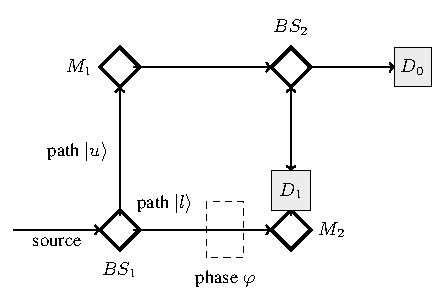
\includegraphics[width=0.82\textwidth]{tikz/mach_zehnder_standalone.pdf}
    \caption{A schematic Mach--Zehnder interferometer. The first beam splitter creates two path alternatives, a phase shifter changes the relative phase, and the second beam splitter recombines the alternatives before detection.}
    \label{fig:mach_zehnder}
\end{figure}

The important feature is that the two alternatives are spatially distinct between the two beam splitters, but the final detection probabilities depend on recombining them. If one blocks either arm, the remaining beam reaches the detectors without interference. If both arms are open, the two possibilities must be considered together. Let $\ket{u}$ and $\ket{l}$ denote the upper and lower paths. A first beam splitter prepares a superposition of paths. In one common convention,
\begin{linenomath}
    \begin{equation}
        \ket{u}\longmapsto
        \frac{1}{\sqrt{2}}\left(\ket{u}+\ket{l}\right).
    \end{equation}
\end{linenomath}
If a phase shifter is placed in the lower arm, the state becomes
\begin{linenomath}
    \begin{equation}
        \ket{\psi}
        =
        \frac{1}{\sqrt{2}}\left(\ket{u}+e^{i\varphi}\ket{l}\right).
    \end{equation}
\end{linenomath}
The phase $\varphi$ does not by itself represent a classical probability. The probabilities of finding the particle in the two arms remain equal before the second beam splitter. Nevertheless, after the paths are recombined, this relative phase changes the final detection probabilities. This is the experimental heart of the device: a phase difference accumulated in one arm, though invisible as an immediate path probability, becomes visible as a redistribution of counts between the two detectors. A second, identical beam splitter recombines the paths. In the convention where each beam splitter acts as $\ket{u}\mapsto(\ket{0}+\ket{1})/\sqrt{2}$ and $\ket{l}\mapsto(\ket{0}-\ket{1})/\sqrt{2}$ on the output-mode basis $\{\ket{0},\ket{1}\}$, the state after recombination is
\begin{linenomath}
    \begin{equation}
        \ket{\psi_{\mathrm{out}}}
        = \frac{1}{2}\Bigl[(1+e^{i\varphi})\ket{0}+(1-e^{i\varphi})\ket{1}\Bigr],
    \end{equation}
\end{linenomath}
and the detection probabilities are
\begin{linenomath}
    \begin{equation}
        P_0=|1+e^{i\varphi}|^{2}/4=(2+2\cos\varphi)/4=\cos^2\frac{\varphi}{2},
        \qquad
        P_1=|1-e^{i\varphi}|^{2}/4=(2-2\cos\varphi)/4=\sin^2\frac{\varphi}{2}.
    \end{equation}
\end{linenomath}
The detector statistics depend on a phase difference between alternatives.

This is the cleanest reason ordinary probability is insufficient. If the particle had merely chosen the upper or lower arm with probability $\frac12,$ the final probability would be an ordinary weighted sum. Changing a phase in one arm would not continuously move counts from one detector to the other. But the experiment requires amplitudes associated with alternatives to be added before the squared modulus is taken. Interference is therefore not a decorative wave effect; it is a rule for composing alternatives.

The same apparatus also clarifies the role of which-path information. If a detector is placed in one arm, or if the two arms are marked in principle by some distinguishable physical trace, the interference disappears. The alternatives then behave more like exclusive classical alternatives. Thus the experiment does not say simply that a particle ``really went both ways'' in an ordinary spatial sense. Rather, it says that when the experimental arrangement does not distinguish the alternatives, the theory must combine their amplitudes before assigning probabilities to final outcomes.

The interferometer is advantageous because it separates two ideas that are often confused: probability and phase. A relative phase can change future probabilities even when it does not change the immediate probabilities for the two paths. The limitation is that the path labels $\ket{u}$ and $\ket{l}$ may tempt one to imagine that the particle really follows one path while the other path is merely a calculational fiction. The interference pattern is precisely the warning against that simplification: the alternatives must be treated together until the experimental arrangement makes them distinguishable.

\subsection{Polarization as a Two-State System}
Polarization is the oldest two-state phenomenon in physics. In 1809 Malus, examining light from a window reflected in a pane of glass through a crystal of Iceland spar, discovered polarization by reflection, together with the law that bears his name: an analyzer transmits the fraction $\cos^2\theta$ of an incident polarized beam, $\theta$ being the angle between the orientations of polarizer and analyzer. Classical wave optics explains the law by the projection of the field vector. For single quanta the situation is sharper: a photon meeting a polarizer has exactly two outcomes, transmitted or absorbed, and Malus' law survives only as a statement of probabilities.

Let $\ket{H}$ and $\ket{V}$ denote horizontal and vertical polarization. These are perfectly distinguishable alternatives for an apparatus that measures polarization in the horizontal-vertical basis. A photon can nevertheless be prepared in a diagonal polarization state
\begin{linenomath}
    \begin{equation}
        \ket{D}=\frac{1}{\sqrt{2}}\left(\ket{H}+\ket{V}\right),
    \end{equation}
\end{linenomath}
or in the anti-diagonal state
\begin{linenomath}
    \begin{equation}
        \ket{A}=\frac{1}{\sqrt{2}}\left(\ket{H}-\ket{V}\right).
    \end{equation}
\end{linenomath}
If a photon in state $\ket{D}$ is measured by a horizontal-vertical polarizing apparatus, the two outcomes occur with equal probability:
\begin{linenomath}
    \begin{equation}
        P(H|D)=|\braket{H|D}|^2=\frac12,\qquad
        P(V|D)=|\braket{V|D}|^2=\frac12.
    \end{equation}
\end{linenomath}
But it would be misleading to say that the photon secretly had either horizontal or vertical polarization before the measurement. The same state $\ket{D}$ is a definite state for a diagonal polarizer. In the diagonal basis it is not a mixture of alternatives; it is one of the basis states.

This is already a departure from the classical notion of state. The question ``what polarization does the photon have?'' is incomplete until one specifies the experimental basis in which the question is asked. Different bases correspond to different decompositions of the same state.

Nothing of this is special to light. Relative to any experiment with two distinguishable outcomes, which we may call $\ket{0}$ and $\ket{1}$ without loss of generality, a general pure state of any quantum system has the form
\begin{linenomath}
    \begin{equation}
        \ket{\psi}=\alpha\ket{0}+\beta\ket{1},
        \qquad |\alpha|^2+|\beta|^2=1.
    \end{equation}
\end{linenomath}
The complex numbers $\alpha$ and $\beta$ are not probabilities themselves. They are \textbf{probability amplitudes}: their squared moduli give the probabilities of the two outcomes in this basis, and their relative phase governs the outcomes of other measurements, as the interferometer has already shown.

For a polarizer oriented at an angle $\theta$ from the horizontal axis, the transmitted polarization state may be written
\begin{linenomath}
    \begin{equation}
        \ket{\theta}=\cos\theta\,\ket{H}+\sin\theta\,\ket{V}.
    \end{equation}
\end{linenomath}
If the incoming photon is horizontally polarized, the transmission probability is
\begin{linenomath}
    \begin{equation}
        P(\theta|H)=|\braket{\theta|H}|^2=\cos^2\theta,
    \end{equation}
\end{linenomath}
which is Malus' law. Thus an elementary optical experiment already suggests the rule: probabilities are squared inner products of state vectors.

The strength of the polarization example is that it makes basis dependence visible with ordinary optical equipment. It also shows why quantum theory cannot be merely a theory of ignorance about a hidden classical alternative. A diagonal polarization is not half horizontal and half vertical in the same sense that a box contains either a red or a blue ball with unknown color. It is a definite preparation that becomes probabilistic only relative to another measurement basis. The limitation of the example is that polarization is often described by classical electromagnetic waves as well; one must be careful not to confuse the classical wave description of a beam with the single-quantum state description of a photon.

\subsection{Sequential Polarizers and the Failure of Boolean Logic}
Consider now three polarizers. If a horizontally polarized beam first meets a vertical polarizer, no light passes in the ideal case:
\begin{linenomath}
    \begin{equation}
        \braket{V|H}=0.
    \end{equation}
\end{linenomath}
Classically, one might expect that inserting an additional filter between them can only reduce the transmitted intensity. But if a diagonal polarizer is placed between the horizontal and vertical polarizers, then some light is transmitted. In the ideal single-photon description, the probability is
\begin{linenomath}
    \begin{equation}
        P(H\to D\to V)
        =
        |\braket{D|H}|^2|\braket{V|D}|^2
        =
        \frac14.
    \end{equation}
\end{linenomath}
The middle polarizer changes the state preparation for the final measurement. It is not merely a passive question about a pre-existing property.

This experiment gives an early warning that the logic of quantum propositions is not simply the Boolean logic of subsets of a classical phase space. The propositions ``horizontal,'' ``vertical,'' and ``diagonal'' are tied to experimental operations, and these operations need not commute. The formal theory will express this noncommutativity through operators, but the phenomenon itself is already visible in elementary polarization experiments.

This is a decisive advantage of the sequential-polarizer experiment. It shows that measurements are not merely windows through which one passively reads pre-existing properties. They can prepare new states. Its limitation, however, is that it still does not display all the drama of quantum mechanics, since absorption by a polarizer may be imagined too mechanically. The Stern--Gerlach experiment below makes the same logical structure harder to dismiss as a peculiarity of light.

\subsection{Stern--Gerlach Experiments and Incompatible Questions}
The Stern--Gerlach experiment, already encountered above as the first direct display of spatial quantization (Section~\ref{subsec:spin}), provides a two-state system not built from light polarization or spatial paths, but from intrinsic angular momentum. The original experiment, performed by Otto Stern and Walther Gerlach in 1922, sent a beam of neutral silver atoms through a strongly inhomogeneous magnetic field. Classically, if the atoms carried tiny magnetic moments pointing in arbitrary directions, the magnetic force should have produced a continuous smear on the detection screen. Instead, the beam split into two separated spots.

\begin{figure}[htbp!]
    \centering
    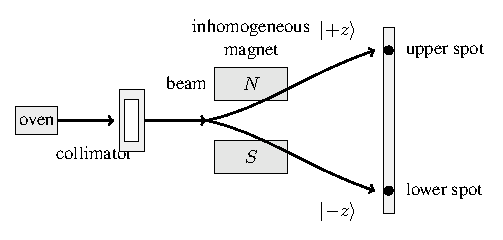
\includegraphics[width=0.86\textwidth]{tikz/stern_gerlach_standalone.pdf}
    \caption{A schematic Stern--Gerlach experiment. A collimated atomic beam passes through an inhomogeneous magnetic field and separates into two discrete beams rather than a continuous spread.}
    \label{fig:stern_gerlach}
\end{figure}

The historical experiment was first interpreted before the modern concept of electron spin had fully crystallized, but in retrospect it displays one of the simplest quantum facts: a component of angular momentum can have discrete outcomes. For a spin-$\frac12$ system measured along the $z$-axis, denote the two possible outcomes by
\begin{linenomath}
    \begin{equation}
        \ket{+z},\qquad \ket{-z}.
    \end{equation}
\end{linenomath}
A particle prepared in $\ket{+z}$ and immediately measured again along $z$ gives the same result with certainty. The first apparatus can therefore be used as a preparation device.

The most revealing form of the experiment is sequential. Send an unpolarized beam through a $z$-oriented Stern--Gerlach apparatus and block the lower output, keeping only the $\ket{+z}$ beam. If this selected beam is sent through a second $z$-oriented apparatus, it does not split again into two equal parts; it goes entirely into the $+z$ output. This shows that the first apparatus has prepared a definite state relative to the same later question.

Now measure the same prepared state along the $x$-axis by rotating the magnetic field gradient. The relevant basis is
\begin{linenomath}
    \begin{equation}
        \ket{+x}=\frac{1}{\sqrt{2}}\left(\ket{+z}+\ket{-z}\right),
        \qquad
        \ket{-x}=\frac{1}{\sqrt{2}}\left(\ket{+z}-\ket{-z}\right).
    \end{equation}
\end{linenomath}
Thus a particle prepared as $\ket{+z}$ gives the two $x$-outcomes with equal probability. More strikingly, if one selects the $\ket{+x}$ beam and then measures $z$ again, the original certainty of the $z$-outcome is lost. The intermediate $x$-measurement has not merely revealed a hidden $x$-property; it has prepared a new state relative to the later $z$-measurement.

\begin{figure}[htbp!]
    \centering
    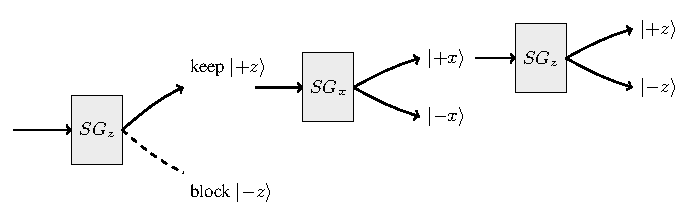
\includegraphics[width=0.95\textwidth]{tikz/sequential_sg_standalone.pdf}
    \caption{Sequential Stern--Gerlach measurements. A $z$-measurement can prepare $\ket{+z}$, but an intervening $x$-measurement destroys the certainty of a later $z$-measurement.}
    \label{fig:sequential_sg}
\end{figure}

The moral is central. The state $\ket{+z}$ is not a catalogue assigning definite values to both $z$-spin and $x$-spin. Instead, it is a rule for assigning amplitudes to possible outcomes in whatever basis an experiment chooses. The incompatibility of different measurement directions is not ignorance in the ordinary sense, but a structural feature of the theory.

The Stern--Gerlach experiment has a special historical and conceptual role because spin is not a disguised position variable. The two outcomes are discrete, reproducible, and associated with spatial direction, yet they cannot be explained as the revelation of a tiny classical arrow with pre-existing components along all axes. The advantage of the spin-$\frac12$ system is therefore its purity: it displays the finite-dimensional Hilbert-space structure without relying on wave motion through two visible arms. Its limitation is that a full account of spin ultimately requires the representation theory of rotations, which will only appear after the general theory of symmetries has been developed.

\subsection{The Operational Meaning of State}
\label{subsec:operational-state}
These three families of experiments --- paths, polarizations, and spin components --- suggest a more careful definition. A physical state should be understood operationally as an equivalence class of preparation procedures: two preparations define the same state if they give the same probabilities for every possible later experiment. This definition does not require us to imagine an unseen list of all properties possessed by the system. It asks only what statistical predictions are reproducibly associated with a preparation.

In the two-state examples, such a preparation is represented by a ray in a complex vector space. Multiplying a vector by an overall nonzero complex number does not change the physical state, since normalized probabilities are unchanged. In particular,
\begin{linenomath}
    \begin{equation}
        \ket{\psi}
        \quad\text{and}\quad
        e^{i\chi}\ket{\psi}
    \end{equation}
\end{linenomath}
represent the same pure state. Relative phases, however, are physically meaningful, as the Mach--Zehnder interferometer shows.

We are thus led to the following preliminary rules:
\begin{enumerate}
    \item mutually distinguishable alternatives are represented by basis vectors;
    \item a general pure state is a linear superposition of these alternatives;
    \item complex amplitudes, not probabilities, are the quantities that combine linearly;
    \item probabilities are obtained from squared moduli of amplitudes;
    \item changing the experimental question corresponds to changing the basis.
\end{enumerate}
These rules are not yet the full Hilbert-space formalism, but they contain its seed. The next chapter will develop this seed systematically, replacing the two-dimensional examples by the general language of vectors, inner products, linear operators, and measurement.
